\chapter{常见多元分布}
\label{chap:multivariate-distributions}

一家甜品店有三种口味，记下接连四位顾客各选了哪一种，得到三个计数；从装着三种颜色小球的盒子里一次摸出四个，也得到三个计数。两台传感器同时测量同一个房间，给出两个可正可负的误差。一份混合物由三种成分组成，三个比例都在$0$与$1$之间，加起来恰好是$1$。这些记录都是随机向量，第~\ref{chap:random-vectors}章已经准备好了描述它们的一般语言：联合分布、边缘、条件、均值向量与协方差矩阵。

可是一般语言不告诉我们具体的概率应当是多少。四位顾客的口味计数取$(2,1,1)$的机会有多大？两台传感器的误差为什么常常一起变大？三个比例能不能各自独立地随机取值？要回答这些问题，需要从试验机制或取值范围出发，写出具体的联合分布，再看它的参数各管什么，分量之间的依赖从哪里来。

本章的五个模型分成三类。计数模型的总数固定，分量之间必然相关，独立重复与不放回抽样又给出不同的协方差。实值观测从多元高斯出发：它由均值向量和协方差矩阵完全确定，边缘、条件和独立性都能用这两个参数直接算出；把它的固定尺度换成所有分量共用的随机尺度，就得到尾部更重的多元t分布和多元Laplace分布。组成比例由Dirichlet分布描述，它住在比例之和为$1$的三角形或更高维单纯形上。

这些模型反复用到同一个问题：知道了每个分量的分布，甚至知道了协方差，能否断定分量之间独立？我们会看到，计数的总和约束、高斯的仿射结构、共同尺度和比例的归一化，各自以不同方式回答它。最后一节把五个模型并排比较。随机变量经过一般映射后的分布、密度换元的完整依据，在第~\ref{chap:random-variable-transformations}章统一处理。

\section{计数分布}
\label{sec:mvd-counting}

先看最朴素的多元记录：每次观察落入$d$个类别之一，观察$n$次，数每一类出现了几次。结果是一个整数向量$\bm{N}=(N_1,\ldots,N_d)^{\top}$，分量非负，并且
\[
 N_1+N_2+\cdots+N_d=n .
\]
这条等式对每一次试验结果都成立，不是平均意义下成立。

本节用两个场景贯穿。第一个是甜品店：每位顾客独立地选口味，选第$1,2,3$种的概率分别是$0.5,0.3,0.2$，记录四位顾客。第二个是摸球：盒子里有$10$个球，其中红球$5$个、绿球$3$个、黄球$2$个，一次不放回地摸出$4$个。两个场景中每一类所占的比例相同，都是$(0.5,0.3,0.2)$，计数总和都是$4$。区别只在一处：顾客之间互不影响，而摸出一个红球会改变盒中剩余的组成。

总和固定这一点已经告诉我们，分量不可能相互独立：若$N_1=4$，其余分量只能是$0$。下面先由试验机制推出两种联合分布，再用示性变量算出它们的均值与协方差，看总和约束和抽样方式分别在协方差里留下什么痕迹。

\subsection{多项分布}
\label{sec:mvd-multinomial}

\paragraph{联合质量函数}
设一个试验重复$n$次，各次相互独立；每次恰好落入$d$个类别之一，落入第$i$类的概率是$p_i$，各次相同。这里$p_i\geq0$，$p_1+\cdots+p_d=1$，记$\bm{p}=(p_1,\ldots,p_d)^{\top}$。用$N_i$表示$n$次中落入第$i$类的次数。

要算$\bm{N}$取某个$\bm{k}=(k_1,\ldots,k_d)^{\top}$的概率，可以先看一条具体的结果序列。例如四位顾客依次选了口味$1,3,1,2$，由独立性，这条序列的概率是各次概率之积，
\[
 p_1\cdot p_3\cdot p_1\cdot p_2=p_1^{2}p_2p_3 .
\]
它只依赖每一类出现了几次，与出现的先后无关。所以$\bm{N}=\bm{k}$的概率等于“计数为$\bm{k}$的序列条数”乘以$\prod_ip_i^{k_i}$。

把$n$个位置分给$d$个类别，第$i$类占$k_i$个位置，分法的数目是多项式系数$n!/(k_1!\cdots k_d!)$：先把$n$个位置全排列，再除去每一类内部位置互换造成的重复。这一计数可参考\BookChapterRef{chap:counting}{卷一第2章“计数”}。合起来得到下面的定义。

\begin{definition}[多项分布]
\label{def:mvd-multinomial}
设$n$为正整数，$\bm{p}$的分量非负且和为$1$。若随机向量$\bm{N}$满足
\begin{equation}
 \mathbb{P}(\bm{N}=\bm{k})=\frac{n!}{k_1!\,k_2!\cdots k_d!}\,p_1^{k_1}p_2^{k_2}\cdots p_d^{k_d},
 \label{eq:mvd-multinomial-pmf}
\end{equation}
其中$\bm{k}$取遍满足$k_i\geq0$、$k_1+\cdots+k_d=n$的整数向量，则称$\bm{N}$服从参数为$n$与$\bm{p}$的\term{多项分布}（multinomial distribution），记为$\bm{N}\sim\operatorname{Mult}(n,\bm{p})$。
\end{definition}

式~\eqref{eq:mvd-multinomial-pmf}的各项之和为$1$，因为按多项式定理，它们恰好是$(p_1+\cdots+p_d)^{n}=1$的展开。$d=2$时，$N_2=n-N_1$由$N_1$决定，式~\eqref{eq:mvd-multinomial-pmf}就是二项分布的质量函数。

回到甜品店，$n=4$，$\bm{p}=(0.5,0.3,0.2)^{\top}$。计数$(2,1,1)$的系数是$4!/(2!\,1!\,1!)=12$，于是
\[
 \mathbb{P}\bigl(\bm{N}=(2,1,1)\bigr)=12\times0.5^{2}\times0.3\times0.2=0.18 .
\]
四位顾客全选第$1$种的概率是$0.5^{4}=0.0625$，全选第$3$种的概率只有$0.2^{4}=0.0016$。

这些概率全部住在一个三角形格点集上。三个计数之和为$4$，可能的取值共有$15$个，把它们画成等边三角形里的格点，三个顶点分别是$(4,0,0)$、$(0,4,0)$和$(0,0,4)$。图~\ref{fig:mvd-count-lattice}(a)用圆的面积表示概率：质量集中在靠近$(2,1,1)$的地方，也就是靠近$n\bm{p}=(2,1.2,0.8)$的地方。三维向量只在一个二维的格点三角形上取值，这正是总和约束的几何形状。

\begin{BookInlineFigure}
  \centering
  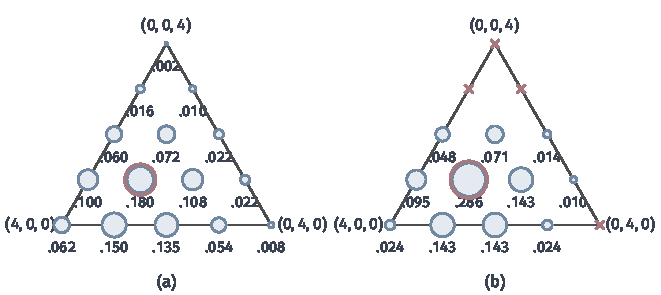
\includegraphics[width=112mm]{figures/07-probability/01-elementary-probability/matplotlib/mvd-count-lattice/figure.pdf}
  \caption{总和为$4$的三类计数的联合分布，每个格点代表一个计数向量$(k_1,k_2,k_3)$，圆的面积与概率成正比，下方数字是概率。(a)多项分布$\operatorname{Mult}(4,(0.5,0.3,0.2))$。(b)从$5$红、$3$绿、$2$黄共$10$个球中不放回摸$4$个的多元超几何分布；红叉是不可能出现的计数。红圈标出$(2,1,1)$。}
  \label{fig:mvd-count-lattice}
\end{BookInlineFigure}

\paragraph{合并类别与边缘分布}
只关心第$1$类时，可以把其余类别合成“非第$1$类”。每次试验仍然相互独立，落入第$1$类的概率仍是$p_1$，所以$N_1$就是$n$次独立试验中的成功次数：
\[
 N_i\sim\operatorname{Bin}(n,p_i),\qquad i=1,\ldots,d .
\]
更一般地，把若干类别合并成一类，合并后的计数仍服从多项分布，参数是对应概率之和。例如甜品店中把口味$1,2$合并，
\[
 (N_1+N_2,\ N_3)\sim\operatorname{Mult}\bigl(4,(0.8,0.2)\bigr) .
\]
这种做法不需要对式~\eqref{eq:mvd-multinomial-pmf}求和，它直接回到试验机制：合并类别只是把记录方式变粗，独立重复的结构没有改变。

\paragraph{示性变量与协方差}
计数的均值和协方差最好通过逐次记录来算。对第$t$次试验和第$i$类，令示性变量
\[
 I_{t,i}=\mathbf{1}_{\{\text{第}t\text{次落入第}i\text{类}\}},\qquad N_i=\sum_{t=1}^{n}I_{t,i} .
\]
把$I_{t,i}$排成$n$行$d$列的表，图~\ref{fig:mvd-indicator-table}画出了序列$1,3,1,2$对应的表，列和就是计数。

\begin{BookInlineFigure}
  \centering
  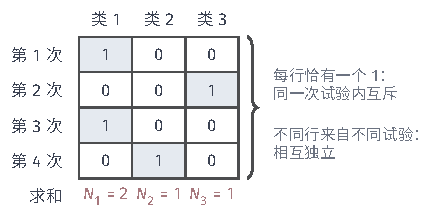
\includegraphics[width=73mm]{figures/07-probability/01-elementary-probability/tikz/mvd-indicator-table/figure.pdf}
  \caption{四次试验、三个类别的示性变量表，对应结果序列$1,3,1,2$。每一行恰有一个$1$（浅蓝），各列之和给出计数$\bm{N}=(2,1,1)$。同一行内的示性变量互斥，不同行来自相互独立的试验。}
  \label{fig:mvd-indicator-table}
\end{BookInlineFigure}

表中有两种关系。同一行的$d$个示性变量互斥：一次试验只能落入一个类别，所以$i\neq j$时$I_{t,i}I_{t,j}=0$。不同行来自不同试验，相互独立。前者产生负的协方差，后者不产生任何交叉项。

\begin{theorem}[多项计数的均值与协方差]
\label{thm:mvd-multinomial-moments}
设$\bm{N}\sim\operatorname{Mult}(n,\bm{p})$，则$\mathbb{E}[\bm{N}]=n\bm{p}$，并且
\begin{equation}
 \operatorname{Cov}(N_i,N_j)=
 \begin{cases}
  np_i(1-p_i), & i=j,\\
  -np_ip_j, & i\neq j .
 \end{cases}
 \label{eq:mvd-multinomial-cov}
\end{equation}
用矩阵写，即
\begin{equation}
 \operatorname{Cov}(\bm{N})=n\bigl(\operatorname{diag}(\bm{p})-\bm{p}\bm{p}^{\top}\bigr) .
 \label{eq:mvd-multinomial-cov-matrix}
\end{equation}
\end{theorem}

\begin{proof}
每个$I_{t,i}$只取$0,1$，取$1$的概率是$p_i$，所以$\mathbb{E}[I_{t,i}]=p_i$，对$t$求和得$\mathbb{E}[N_i]=np_i$。

协方差对两个变量都是线性的，展开两个和式，
\[
 \operatorname{Cov}(N_i,N_j)=\sum_{t=1}^{n}\sum_{s=1}^{n}\operatorname{Cov}(I_{t,i},I_{s,j}) .
\]
$t\neq s$时两个示性变量来自不同试验，相互独立，协方差为$0$。只剩$t=s$的$n$项。

同一次试验中，$i=j$时$I_{t,i}^{2}=I_{t,i}$；$i\neq j$时$I_{t,i}I_{t,j}=0$。于是
\[
 \operatorname{Cov}(I_{t,i},I_{t,j})=\mathbb{E}[I_{t,i}I_{t,j}]-p_ip_j=
 \begin{cases}
  p_i-p_i^{2}, & i=j,\\
  -p_ip_j, & i\neq j .
 \end{cases}
\]
乘以$n$即得式~\eqref{eq:mvd-multinomial-cov}。
\end{proof}

对甜品店，$n=4$，$\bm{p}=(0.5,0.3,0.2)^{\top}$，代入式~\eqref{eq:mvd-multinomial-cov}，协方差矩阵是
\[
 \begin{bmatrix}
  1 & -0.6 & -0.4\\
  -0.6 & 0.84 & -0.24\\
  -0.4 & -0.24 & 0.64
 \end{bmatrix} .
\]
对角元是三个二项分布的方差，非对角元全为负：一位顾客选了口味$1$，就不能再选口味$2$。

这个矩阵每一行的和都是$0$。一般地，第$i$行之和为$np_i-np_i\sum_jp_j=0$，即协方差矩阵乘以全一向量$\bm{1}$得零向量。这与总和约束一致：
\[
 \operatorname{Var}(N_1+\cdots+N_d)=\bm{1}^{\top}\operatorname{Cov}(\bm{N})\bm{1}=0 ,
\]
常数$n$没有波动。所以多项分布的协方差矩阵总是奇异的。

当各$p_i>0$时，$\bm{1}$的倍数是零空间中仅有的方向。若式~\eqref{eq:mvd-multinomial-cov-matrix}的矩阵把$\bm{v}$映成零向量，第$i$个分量给出$p_iv_i=p_i(\bm{p}^{\top}\bm{v})$，除以$p_i$得$v_i=\bm{p}^{\top}\bm{v}$，各分量相等。因此协方差矩阵的秩是$d-1$，与格点三角形的维数相同。

负协方差说明分量相关，因而不独立。也可以直接看一个事件：$\mathbb{P}(N_1=4)=0.0625$，$\mathbb{P}(N_2=4)=0.0081$，两者都为正，可是$N_1=4$与$N_2=4$不能同时发生，联合概率是$0$，不等于乘积。把各类计数当成独立的二项变量，会给不可能的组合分配正概率。

\subsection{多元超几何分布}
\label{sec:mvd-multivariate-hypergeometric}

\paragraph{联合质量函数}
现在换成摸球。总体有$M$个对象，第$i$类有$K_i$个，$K_1+\cdots+K_d=M$；从中一次不放回地取出$n$个，$1\leq n\leq M$，每个$n$元子集被取到的机会相同。仍用$N_i$记取出的第$i$类个数。

所有可能的子集共有$\binom{M}{n}$个。取出的结果恰好含$k_i$个第$i$类对象，相当于在每一类里各自挑$k_i$个，挑法数相乘，于是得到下面的定义。

\begin{definition}[多元超几何分布]
\label{def:mvd-multivariate-hypergeometric}
设各类数目$K_i$为非负整数，$M=\sum_iK_i$，$1\leq n\leq M$。若
\begin{equation}
 \mathbb{P}(\bm{N}=\bm{k})=\frac{\binom{K_1}{k_1}\binom{K_2}{k_2}\cdots\binom{K_d}{k_d}}{\binom{M}{n}},
 \label{eq:mvd-mhyper-pmf}
\end{equation}
其中$\bm{k}$取遍满足$0\leq k_i\leq K_i$、$k_1+\cdots+k_d=n$的整数向量，则称$\bm{N}$服从\term{多元超几何分布}（multivariate hypergeometric distribution）。
\end{definition}

与多项分布相比，取值多了上限$k_i\leq K_i$：盒子里只有$2$个黄球，就不可能摸出$3$个。在摸球例子中，$M=10$，$\bm{K}=(5,3,2)$，$n=4$，$\binom{10}{4}=210$。计数$(2,1,1)$的概率是
\[
 \frac{\binom{5}{2}\binom{3}{1}\binom{2}{1}}{210}=\frac{10\times3\times2}{210}=\frac{2}{7}\approx0.286 ,
\]
比多项分布的$0.18$大。图~\ref{fig:mvd-count-lattice}(b)画出全部格点：黄球数为$3$或$4$、绿球数为$4$的格点概率为$0$，用红叉标出；剩下的质量更集中在中间。

\paragraph{逐次抽取的对称性}
求均值和协方差时，把“一次取出$n$个”想成依次取出$n$个、每次在剩下的对象中等可能地取一个。这样得到的有序结果共有$M(M-1)\cdots(M-n+1)$种，每种机会相同，忽略顺序就回到等可能的子集。仍记$I_{t,i}$为第$t$次取到第$i$类的示性变量，$N_i=\sum_tI_{t,i}$。

关键是一个对称性：第$t$次取到的对象在全体$M$个对象上等可能。数一数就知道：指定第$t$次取对象$o$，其余$n-1$个位置从剩下的$M-1$个对象中依次挑选，有序结果的条数与$o$是哪一个无关。同理，对$t\neq s$，第$t$次与第$s$次取到的有序对在所有$M(M-1)$个“不同对象的有序对”上等可能。

记$q_i=K_i/M$为第$i$类的比例。由第一条对称性，$\mathbb{P}(I_{t,i}=1)=q_i$。由第二条，$t\neq s$时，
\[
 \mathbb{P}(I_{t,i}=1,\ I_{s,j}=1)=
 \begin{cases}
  \dfrac{K_i(K_i-1)}{M(M-1)}, & i=j,\\
  \dfrac{K_iK_j}{M(M-1)}, & i\neq j .
 \end{cases}
\]
这里需要$M\geq2$。不同次的抽取不再独立：先取走一个第$i$类对象，第$i$类在剩余对象中的比例就变小了。

\begin{theorem}[多元超几何计数的均值与协方差]
\label{thm:mvd-mhyper-moments}
设$\bm{N}$服从定义~\ref{def:mvd-multivariate-hypergeometric}的分布，$M\geq2$，$\bm{q}=\bm{K}/M$。则$\mathbb{E}[\bm{N}]=n\bm{q}$，并且
\begin{equation}
 \operatorname{Cov}(\bm{N})=n\,\frac{M-n}{M-1}\bigl(\operatorname{diag}(\bm{q})-\bm{q}\bm{q}^{\top}\bigr) .
 \label{eq:mvd-mhyper-cov}
\end{equation}
\end{theorem}

\begin{proof}
均值由$\mathbb{E}[I_{t,i}]=q_i$对$t$求和得到。协方差仍按双重和展开，分成$t=s$的$n$项和$t\neq s$的$n(n-1)$项。同一次抽取内的情形与多项分布完全一样，贡献$n(\delta_{i,j}q_i-q_iq_j)$，其中$\delta_{i,j}$在$i=j$时为$1$、否则为$0$。

先算$i\neq j$。由上面的联合概率，$t\neq s$的每一项是
\[
 \frac{K_iK_j}{M(M-1)}-q_iq_j=q_iq_j\Bigl(\frac{M}{M-1}-1\Bigr)=\frac{q_iq_j}{M-1} .
\]
两部分相加，
\[
 \operatorname{Cov}(N_i,N_j)=-nq_iq_j+\frac{n(n-1)q_iq_j}{M-1}=-nq_iq_j\,\frac{M-n}{M-1} .
\]

再算$i=j$。$t\neq s$的每一项是
\[
 \frac{K_i(K_i-1)}{M(M-1)}-q_i^{2}=q_i\,\frac{(K_i-1)M-K_i(M-1)}{M(M-1)}=-\frac{q_i(1-q_i)}{M-1} .
\]
与$t=s$的贡献$nq_i(1-q_i)$相加，
\[
 \operatorname{Var}(N_i)=nq_i(1-q_i)\Bigl(1-\frac{n-1}{M-1}\Bigr)=nq_i(1-q_i)\,\frac{M-n}{M-1} .
\]
两种情形合起来就是式~\eqref{eq:mvd-mhyper-cov}。
\end{proof}

\paragraph{与多项分布的比较}
取多项分布的$\bm{p}$等于总体比例$\bm{q}$，两种抽样的均值完全相同，协方差的形状也相同，只差一个因子$(M-n)/(M-1)$。$n\geq2$时这个因子小于$1$：不放回抽样的计数波动更小。直观上，摸出一个红球后剩下的红球变少，下一次摸到红球的机会随之下降，这种负反馈把计数往总体比例上拉。

摸球例子中，因子是$(10-4)/(10-1)=2/3$。红球数的方差从多项分布的$1$降到$2/3$，红、绿两类的协方差从$-0.6$变成$-0.4$。极端情形$n=M$时因子为$0$：整盒取出，计数恒等于$\bm{K}$，没有任何随机性。$n=1$时因子为$1$，一次抽取放回与否没有区别。

总和约束对两种模型同样起作用。$\operatorname{diag}(\bm{q})-\bm{q}\bm{q}^{\top}$的行和为$0$，所以式~\eqref{eq:mvd-mhyper-cov}同样是奇异矩阵，各类计数两两负相关。

\paragraph{何时可以用多项分布近似}
直观上，总体很大而只取少数几个时，取走的对象几乎不改变剩余组成，不放回与放回应当相差无几。下面的结论把这一点说准确。

\begin{theorem}[大总体下的多项近似]
\label{thm:mvd-mhyper-limit}
固定$n$、$d$和满足$\sum_ik_i=n$的非负整数向量$\bm{k}$。让总体规模$M\to\infty$，各类数目$K_i=K_i(M)$满足$K_i/M\to q_i$，则式~\eqref{eq:mvd-mhyper-pmf}的概率趋于$\operatorname{Mult}(n,\bm{q})$在$\bm{k}$处的概率。
\end{theorem}

\begin{proof}
把二项式系数写成阶乘之比，式~\eqref{eq:mvd-mhyper-pmf}改写为
\[
 \frac{n!}{k_1!\cdots k_d!}\cdot
 \frac{\prod_{i=1}^{d}K_i(K_i-1)\cdots(K_i-k_i+1)}{M(M-1)\cdots(M-n+1)} .
\]
第一个因子就是多项式系数。第二个因子的分子共有$\sum_ik_i=n$个因子，分母也是$n$个因子。

把分子分母的因子一一配对，每一对形如$(K_i-a)/(M-b)$，其中$a<k_i$、$b<n$都是固定整数。$M\to\infty$时，
\[
 \frac{K_i-a}{M-b}=\frac{K_i/M-a/M}{1-b/M}\to q_i .
\]
第$i$类恰好贡献$k_i$对，所以第二个因子趋于$\prod_iq_i^{k_i}$，与第一个因子相乘即为式~\eqref{eq:mvd-multinomial-pmf}。
\end{proof}

定理只说极限，实际使用时还要看差多少。协方差的因子$(M-n)/(M-1)$与$1-n/M$相差不到$1/(M-1)$，所以抽样比例$n/M$是主要的判断依据。图~\ref{fig:mvd-hypergeom-approx}保持红球比例$0.5$、$n=4$：$M=10$时红球数的分布明显比$\operatorname{Bin}(4,0.5)$集中，$M=40$时已经相当接近。右图说明方差因子几乎落在直线$1-n/M$上。

\begin{BookInlineFigure}
  \centering
  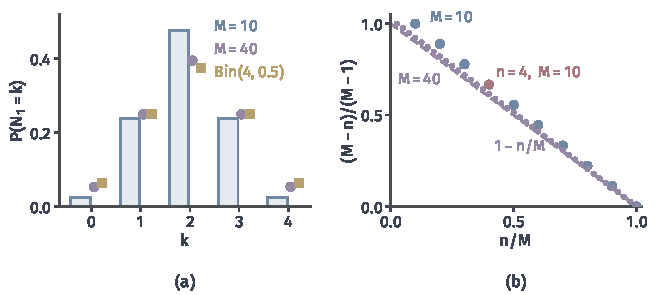
\includegraphics[width=112mm]{figures/07-probability/01-elementary-probability/matplotlib/mvd-hypergeom-approx/figure.pdf}
  \caption{不放回与放回抽样的比较，第$1$类比例$0.5$，抽取$n=4$个。(a)第$1$类计数$N_1$的质量函数：总体$M=10$（蓝色柱）、$M=40$（紫点）与$\operatorname{Bin}(4,0.5)$（黄色方块）。(b)方差因子$(M-n)/(M-1)$随抽样比例$n/M$的变化，蓝点为$M=10$，紫点为$M=40$，紫色虚线为$1-n/M$；红点是本节例子$n=4$、$M=10$。}
  \label{fig:mvd-hypergeom-approx}
\end{BookInlineFigure}

具体数值是：$M=10$时$\mathbb{P}(N_1=2)=100/210\approx0.476$，$M=40$时约为$0.395$，二项分布为$6/16=0.375$。抽样比例从$0.4$降到$0.1$，差距从$0.10$缩小到$0.02$。抽样比例不小时，应当保留有限总体的结构，否则会高估计数的波动，还会给超出$K_i$的计数分配概率。


\section{多元高斯分布}
\label{sec:mvd-gaussian}

两台传感器测量同一房间的温度，各自有测量误差。误差由许多小扰动叠加而成，其中有的扰动只影响一台传感器，比如各自电路的噪声；有的同时影响两台，比如房间里的气流。设三个扰动$Z_1,Z_2,Z_3$相互独立，都服从$\mathcal{N}(0,1)$，第一台读数受$Z_1,Z_2$影响，第二台受$Z_2,Z_3$影响：
\[
 X_1=2+Z_1+Z_2,\qquad X_2=1+Z_2+Z_3 .
\]
两个读数共享$Z_2$，所以一起偏高、一起偏低的机会更大。

这个例子已经包含了多元高斯分布的构造方式：从独立的标准高斯变量出发，做一次仿射变换。一元时，$\mathcal{N}(\mu,\sigma^{2})$就是$\mu+\sigma Z$的分布；多元时，把$\sigma$换成矩阵。本节先说明这样构造出的分布只由均值向量和协方差矩阵决定，再在两个小节中研究它的支撑与密度、条件分布与独立性。由样本估计$\bm{\mu}$与$\bm{\Sigma}$属于统计推断，归卷八处理。

\paragraph{标准高斯向量}
设$Z_1,\ldots,Z_k$相互独立，都服从$\mathcal{N}(0,1)$，记$\bm{Z}=(Z_1,\ldots,Z_k)^{\top}$，称为$k$维标准高斯向量，记为$\bm{Z}\sim\mathcal{N}(\bm{0},\bm{I}_k)$。独立变量的联合密度是边缘密度之积，
\[
 \varphi_k(\bm{z})=\prod_{i=1}^{k}\frac{1}{\sqrt{2\pi}}\mathrm{e}^{-z_i^{2}/2}=\frac{1}{(2\pi)^{k/2}}\mathrm{e}^{-\lVert\bm{z}\rVert_2^{2}/2} .
\]
这个密度只依赖$\bm{z}$到原点的距离，等密度线是同心球面。由此得到一个后面反复要用的事实：把标准高斯向量旋转一下，分布不变。

\begin{lemma}[旋转不变性]
\label{lem:mvd-rotation}
设$\bm{Z}\sim\mathcal{N}(\bm{0},\bm{I}_k)$。若$\bm{Q}$是$k\times k$正交矩阵，则$\bm{Q}\bm{Z}$与$\bm{Z}$同分布。若$r\times k$矩阵$\bm{C}$满足$\bm{C}\bm{C}^{\top}=\bm{I}_r$，则$\bm{C}\bm{Z}\sim\mathcal{N}(\bm{0},\bm{I}_r)$。
\end{lemma}

\begin{proof}
对$\mathbb{R}^{k}$中的区域$S$，事件$\bm{Q}\bm{Z}\in S$就是$\bm{Z}\in\bm{Q}^{\top}S$，所以
\[
 \mathbb{P}(\bm{Q}\bm{Z}\in S)=\int_{\bm{Q}^{\top}S}\varphi_k(\bm{z})\,\mathrm{d}\bm{z} .
\]
作线性换元$\bm{z}=\bm{Q}^{\top}\bm{x}$，积分区域变回$S$，Jacobian行列式的绝对值是$\lvert\det\bm{Q}^{\top}\rvert=1$（换元公式可参考\BookChapterRef{chap:region-integrals}{卷二第24章“区域积分”}）。又$\bm{Q}^{\top}$保持向量的长度，被积函数不变，于是
\[
 \mathbb{P}(\bm{Q}\bm{Z}\in S)=\int_{S}\varphi_k(\bm{x})\,\mathrm{d}\bm{x}=\mathbb{P}(\bm{Z}\in S) .
\]

对第二个结论，$\bm{C}$的$r$行是$\mathbb{R}^{k}$中的标准正交向量组，可以补成一组标准正交基，排成正交矩阵$\bm{Q}$，其前$r$行就是$\bm{C}$。由第一部分，$\bm{Q}\bm{Z}$是标准高斯向量，它的$k$个分量相互独立且都服从$\mathcal{N}(0,1)$。$\bm{C}\bm{Z}$是其中前$r$个分量，自然也是这样。
\end{proof}

\paragraph{仿射构造}
设$\bm{A}$是$d\times k$矩阵，$\bm{\mu}\in\mathbb{R}^{d}$，令$\bm{X}=\bm{\mu}+\bm{A}\bm{Z}$。由期望的线性性，$\mathbb{E}[\bm{X}]=\bm{\mu}$；由第~\ref{chap:random-vectors}章协方差矩阵的线性变换规则，
\[
 \operatorname{Cov}(\bm{X})=\bm{A}\operatorname{Cov}(\bm{Z})\bm{A}^{\top}=\bm{A}\bm{A}^{\top} .
\]
开头的传感器例子中，$\bm{\mu}=(2,1)^{\top}$，$k=3$，
\[
 \bm{A}=\begin{bmatrix}1&1&0\\0&1&1\end{bmatrix},\qquad
 \bm{A}\bm{A}^{\top}=\begin{bmatrix}2&1\\1&2\end{bmatrix} .
\]
非对角元$1$正是共享的$Z_2$贡献的方差。

同一个协方差矩阵可以由许多不同的$\bm{A}$得到。例如二阶方阵
\[
 \bm{L}=\begin{bmatrix}\sqrt2&0\\1/\sqrt2&\sqrt{3/2}\end{bmatrix}
\]
也满足$\bm{L}\bm{L}^{\top}=\bm{A}\bm{A}^{\top}$，它是Cholesky因子；对称平方根$\bm{\Sigma}^{1/2}$是另一个选择。用“三个扰动”还是“两个扰动”来生成，得到的读数分布会不会不同？下面的定理说不会：分布只认$\bm{\mu}$和$\bm{A}\bm{A}^{\top}$。

\begin{theorem}[多元高斯由均值与协方差确定]
\label{thm:mvd-gaussian-well-defined}
设$\bm{Z}\sim\mathcal{N}(\bm{0},\bm{I}_k)$，$\bm{Z}'\sim\mathcal{N}(\bm{0},\bm{I}_{k'})$，$\bm{A}$、$\bm{A}'$分别是$d\times k$与$d\times k'$矩阵。若$\bm{A}\bm{A}^{\top}=\bm{A}'\bm{A}'^{\top}$，则$\bm{\mu}+\bm{A}\bm{Z}$与$\bm{\mu}+\bm{A}'\bm{Z}'$同分布。并且每个$d\times d$对称半正定矩阵$\bm{\Sigma}$都能写成某个$\bm{A}\bm{A}^{\top}$。
\end{theorem}

\begin{proof}
记$\bm{\Sigma}=\bm{A}\bm{A}^{\top}$，秩为$r$。由谱分解（可参考\BookChapterRef{chap:eigen-spectral-decomposition}{卷二第6章“谱分解”}），
\[
 \bm{\Sigma}=\sum_{i=1}^{r}\lambda_i\bm{v}_i\bm{v}_i^{\top},\qquad \lambda_i>0,\ \bm{v}_i\text{标准正交} .
\]
令$\bm{B}$的第$i$列为$\sqrt{\lambda_i}\bm{v}_i$，则$\bm{B}$是$d\times r$矩阵，列满秩，$\bm{B}\bm{B}^{\top}=\bm{\Sigma}$。我们证明$\bm{A}\bm{Z}$与$\bm{B}\bm{W}$同分布，其中$\bm{W}\sim\mathcal{N}(\bm{0},\bm{I}_r)$；$\bm{A}'$同理，两者便同分布。

第一步，$\bm{A}$与$\bm{\Sigma}$的列空间相同。由$\bm{\Sigma}\bm{y}=\bm{A}(\bm{A}^{\top}\bm{y})$，$\bm{\Sigma}$的列空间含于$\bm{A}$的列空间。反过来，若$\bm{v}$与$\bm{\Sigma}$的列空间正交，则$\bm{\Sigma}\bm{v}=\bm{0}$，于是
\[
 \lVert\bm{A}^{\top}\bm{v}\rVert_2^{2}=\bm{v}^{\top}\bm{\Sigma}\bm{v}=0 ,
\]
$\bm{v}$也与$\bm{A}$的列正交。两个列空间的正交补相同，所以列空间相同，也都等于$\bm{B}$的列空间。

第二步，把$\bm{A}$写成$\bm{B}\bm{C}$。$\bm{B}$列满秩，$\bm{B}^{\top}\bm{B}$可逆，令
\[
 \bm{B}^{+}=(\bm{B}^{\top}\bm{B})^{-1}\bm{B}^{\top} ,
\]
则$\bm{B}^{+}\bm{B}=\bm{I}_r$，而$\bm{B}\bm{B}^{+}$是到$\bm{B}$列空间的正交投影。$\bm{A}$的列都在这个空间里，所以
\[
 \bm{A}=\bm{B}\bm{B}^{+}\bm{A}=\bm{B}\bm{C},\qquad \bm{C}=\bm{B}^{+}\bm{A} .
\]

第三步，$\bm{C}$的行标准正交。直接计算，
\[
 \bm{C}\bm{C}^{\top}=\bm{B}^{+}\bm{A}\bm{A}^{\top}(\bm{B}^{+})^{\top}=\bm{B}^{+}\bm{B}\bm{B}^{\top}(\bm{B}^{+})^{\top}=\bm{I}_r .
\]
由引理~\ref{lem:mvd-rotation}，$\bm{C}\bm{Z}\sim\mathcal{N}(\bm{0},\bm{I}_r)$，于是$\bm{A}\bm{Z}=\bm{B}(\bm{C}\bm{Z})$与$\bm{B}\bm{W}$同分布。

最后，半正定矩阵$\bm{\Sigma}$的谱分解中$\lambda_i\geq0$，上面构造的$\bm{B}$就满足$\bm{B}\bm{B}^{\top}=\bm{\Sigma}$。
\end{proof}

证明的想法是：不同的$\bm{A}$只相差一次“旋转”，而标准高斯向量对旋转不敏感。传感器例子中，三个扰动经过$\bm{C}$压成两个独立的标准高斯变量，信息上没有丢失任何影响读数的东西。有了这个定理，下面的定义才有意义。

\begin{definition}[多元高斯分布]
\label{def:mvd-gaussian}
设$\bm{\mu}\in\mathbb{R}^{d}$，$\bm{\Sigma}$是$d\times d$对称半正定矩阵。若随机向量$\bm{X}$与$\bm{\mu}+\bm{A}\bm{Z}$同分布，其中$\bm{Z}\sim\mathcal{N}(\bm{0},\bm{I}_k)$，$\bm{A}$为满足
\begin{equation}
 \bm{A}\bm{A}^{\top}=\bm{\Sigma}
 \label{eq:mvd-gaussian-factor}
\end{equation}
的$d\times k$矩阵，则称$\bm{X}$服从均值为$\bm{\mu}$、协方差矩阵为$\bm{\Sigma}$的\term{多元高斯分布}（multivariate Gaussian distribution），记为$\bm{X}\sim\mathcal{N}(\bm{\mu},\bm{\Sigma})$，也说$\bm{X}$的分量\term{联合高斯}（jointly Gaussian）。
\end{definition}

这里$\bm{\Sigma}$是粗体大写的矩阵，与求和号无关。传感器例子中$\bm{X}\sim\mathcal{N}(\bm{\mu},\bm{\Sigma})$，$\bm{\mu}=(2,1)^{\top}$，$\bm{\Sigma}$的对角元为$2$、非对角元为$1$，本节一直用这组参数。图~\ref{fig:mvd-gauss-affine}把$400$个标准高斯点经过$\bm{x}=\bm{\mu}+\bm{\Sigma}^{1/2}\bm{z}$映过去：圆被拉成斜放的椭圆，点云随之倾斜。

\begin{BookInlineFigure}
  \centering
  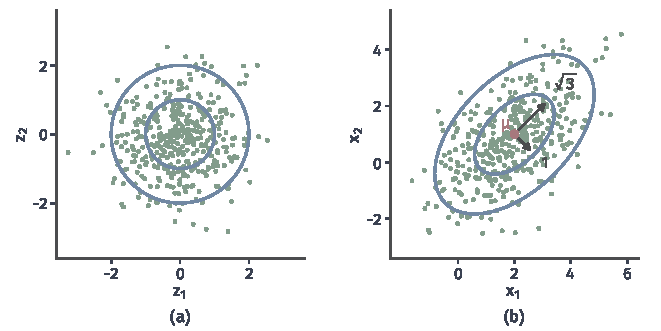
\includegraphics[width=112mm]{figures/07-probability/01-elementary-probability/matplotlib/mvd-gauss-affine/figure.pdf}
  \caption{仿射构造。(a)$400$个二维标准高斯点（绿，种子$7$）与半径$1$、$2$的圆（蓝）。(b)同一批点经$\bm{x}=\bm{\mu}+\bm{\Sigma}^{1/2}\bm{z}$映射后的位置，$\bm{\mu}=(2,1)^{\top}$（红点），$\Sigma_{1,1}=\Sigma_{2,2}=2$，$\Sigma_{1,2}=1$；圆变成椭圆，箭头是两条主轴方向，半轴长分别为$\sqrt3$与$1$。}
  \label{fig:mvd-gauss-affine}
\end{BookInlineFigure}

\paragraph{仿射变换与边缘分布}
构造方式本身就是仿射变换，所以再做一次仿射变换，结果仍是多元高斯。设$\bm{X}\sim\mathcal{N}(\bm{\mu},\bm{\Sigma})$，$\bm{M}$是$m\times d$矩阵，$\bm{c}\in\mathbb{R}^{m}$。把$\bm{X}$写成$\bm{\mu}+\bm{A}\bm{Z}$，
\[
 \bm{M}\bm{X}+\bm{c}=(\bm{M}\bm{\mu}+\bm{c})+(\bm{M}\bm{A})\bm{Z},\qquad (\bm{M}\bm{A})(\bm{M}\bm{A})^{\top}=\bm{M}\bm{\Sigma}\bm{M}^{\top} .
\]由定义~\ref{def:mvd-gaussian}，
\begin{equation}
 \bm{M}\bm{X}+\bm{c}\sim\mathcal{N}\bigl(\bm{M}\bm{\mu}+\bm{c},\ \bm{M}\bm{\Sigma}\bm{M}^{\top}\bigr) .
 \label{eq:mvd-gaussian-affine}
\end{equation}
这里不要求$\bm{M}$满秩，也不要求$m\leq d$。

两种特殊的$\bm{M}$最常用。取$\bm{M}$为单位矩阵的若干行，$\bm{M}\bm{X}$就是$\bm{X}$的一部分分量，于是边缘分布不必积分，只要从$\bm{\mu}$和$\bm{\Sigma}$中取出对应的子向量和子矩阵。取$\bm{M}=\bm{a}^{\top}$，得到一元线性组合
\[
 \bm{a}^{\top}\bm{X}\sim\mathcal{N}(\bm{a}^{\top}\bm{\mu},\ \bm{a}^{\top}\bm{\Sigma}\bm{a}) .
\]
方差为$0$时，$\mathcal{N}(m,0)$理解为恒取$m$的退化分布。

传感器例子中，$X_1\sim\mathcal{N}(2,2)$，$X_2\sim\mathcal{N}(1,2)$。两台读数之和与之差分别是
\[
 \begin{aligned}
  X_1+X_2&\sim\mathcal{N}(3,\,2+2+2\times1)=\mathcal{N}(3,6),\\
  X_1-X_2&\sim\mathcal{N}(1,\,2+2-2\times1)=\mathcal{N}(1,2) .
 \end{aligned}
\]
共享的扰动在和里叠加，在差里抵消，所以差的方差比和小。

\subsection{协方差与支撑}
\label{sec:mvd-gaussian-support}

定义~\ref{def:mvd-gaussian}只要求$\bm{\Sigma}$半正定。$\bm{\Sigma}$正定时，分布铺满整个$\mathbb{R}^{d}$，有普通的$d$维密度；$\bm{\Sigma}$奇异时，分布挤在一个低维的平面里。下面分别看这两种情形，再说明怎样判断一个随机向量是不是联合高斯。

\paragraph{正定协方差与密度}
$\bm{\Sigma}$正定时可以取方阵$\bm{A}$。例如Cholesky分解$\bm{\Sigma}=\bm{L}\bm{L}^{\top}$给出可逆的下三角矩阵$\bm{L}$（可参考\BookChapterRef{chap:direct-linear-solvers}{卷二第12章“线性方程的直接求解”}）。于是$\bm{X}=\bm{\mu}+\bm{L}\bm{Z}$是对标准高斯向量做可逆仿射变换，可以把$\bm{Z}$的密度搬过来。

\begin{theorem}[多元高斯密度]
\label{thm:mvd-gaussian-density}
设$\bm{\Sigma}$正定，$\bm{X}\sim\mathcal{N}(\bm{\mu},\bm{\Sigma})$，则$\bm{X}$有联合密度
\begin{equation}
 f_{\bm{X}}(\bm{x})=\frac{1}{(2\pi)^{d/2}(\det\bm{\Sigma})^{1/2}}\exp\Bigl(-\frac12Q(\bm{x})\Bigr),\qquad \bm{x}\in\mathbb{R}^{d},
 \label{eq:mvd-gaussian-density}
\end{equation}
其中
\begin{equation}
 Q(\bm{x})=(\bm{x}-\bm{\mu})^{\top}\bm{\Sigma}^{-1}(\bm{x}-\bm{\mu}) .
 \label{eq:mvd-gaussian-quadratic}
\end{equation}
\end{theorem}

\begin{proof}
对区域$S$，事件$\bm{X}\in S$就是$\bm{Z}\in\bm{L}^{-1}(S-\bm{\mu})$，所以
\[
 \mathbb{P}(\bm{X}\in S)=\int_{\bm{L}^{-1}(S-\bm{\mu})}\varphi_d(\bm{z})\,\mathrm{d}\bm{z} .
\]
作线性换元$\bm{z}=\bm{L}^{-1}(\bm{x}-\bm{\mu})$，积分区域变成$S$，体积元变为$\lvert\det\bm{L}^{-1}\rvert\,\mathrm{d}\bm{x}$。由$\det\bm{\Sigma}=(\det\bm{L})^{2}$，
\[
 \lvert\det\bm{L}^{-1}\rvert=(\det\bm{\Sigma})^{-1/2} .
\]
又$\bm{L}^{-\top}\bm{L}^{-1}=\bm{\Sigma}^{-1}$，所以$\lVert\bm{z}\rVert_2^{2}=Q(\bm{x})$。代入即得：$\bm{X}$落在$S$中的概率等于$f_{\bm{X}}$在$S$上的积分。
\end{proof}

公式的两部分各有来历。指数里的$Q(\bm{x})$是把偏离量$\bm{x}-\bm{\mu}$“还原”成标准高斯坐标后的平方长度；前面的$(\det\bm{\Sigma})^{-1/2}$是体积的缩放：$\bm{L}$把单位体积拉成$\det\bm{L}$倍，同样多的概率摊在更大的体积上，密度就按同一倍数降低。$d=1$时$Q=(x-\mu)^{2}/\sigma^{2}$，回到一元高斯密度。证明中的线性换元在第~\ref{chap:random-variable-transformations}章发展为一般的密度换元公式。

传感器例子中，$\det\bm{\Sigma}=3$，
\[
 \bm{\Sigma}^{-1}=\frac13\begin{bmatrix}2&-1\\-1&2\end{bmatrix} .
\]
记$u_1=x_1-2$，$u_2=x_2-1$，则$Q=\tfrac23(u_1^{2}-u_1u_2+u_2^{2})$，密度为
\[
 f_{\bm{X}}(\bm{x})=\frac{1}{2\sqrt3\,\pi}\exp\Bigl(-\frac{u_1^{2}-u_1u_2+u_2^{2}}{3}\Bigr) .
\]
在$\bm{x}=\bm{\mu}$处取最大值$1/(2\sqrt3\,\pi)\approx0.0919$。

\paragraph{等密度椭球与马氏距离}
密度只通过$Q(\bm{x})$依赖$\bm{x}$，等密度集是$Q(\bm{x})=c^{2}$。用谱分解
\[
 \bm{\Sigma}=\sum_{i=1}^{d}\lambda_i\bm{v}_i\bm{v}_i^{\top},\qquad \bm{\Sigma}^{-1}=\sum_{i=1}^{d}\lambda_i^{-1}\bm{v}_i\bm{v}_i^{\top},
\]
在以$\bm{\mu}$为原点、以$\bm{v}_i$为坐标轴的坐标$y_i=\bm{v}_i^{\top}(\bm{x}-\bm{\mu})$下，
\[
 Q(\bm{x})=\sum_{i=1}^{d}\frac{y_i^{2}}{\lambda_i} .
\]
所以$Q=c^{2}$是以$\bm{\mu}$为中心的椭球，主轴沿特征向量$\bm{v}_i$，半轴长为$c\sqrt{\lambda_i}$。方差大的方向椭球长，方差小的方向椭球扁。

量$\sqrt{Q(\bm{x})}$称为$\bm{x}$到$\bm{\mu}$的\term{马氏距离}（Mahalanobis distance）。它按各方向的波动大小度量偏离：沿方差大的方向走一段距离，算作较小的偏离。传感器例子的特征值是$3$和$1$，对应方向$(1,1)^{\top}/\sqrt2$与$(1,-1)^{\top}/\sqrt2$。两台读数同向偏离较常见，反向偏离较少见。

取两点$\bm{a}=\bm{\mu}+(1,1)^{\top}$和$\bm{b}=\bm{\mu}+(1,-1)^{\top}$，它们到$\bm{\mu}$的欧氏距离都是$\sqrt2$。代入$Q$，
\[
 Q(\bm{a})=\tfrac23(1-1+1)=\tfrac23,\qquad Q(\bm{b})=\tfrac23(1+1+1)=2 .
\]
两者相差$4/3$，密度之比为$\mathrm{e}^{2/3}\approx1.95$。图~\ref{fig:mvd-gauss-mahalanobis}(a)中，$\bm{a}$落在较内的椭圆上，$\bm{b}$落在较外的椭圆上，尽管两者在同一个欧氏圆上。

\begin{BookInlineFigure}
  \centering
  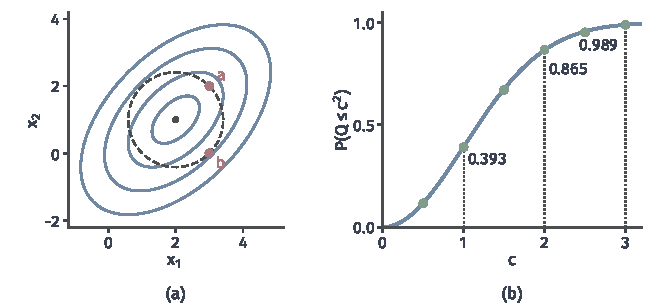
\includegraphics[width=112mm]{figures/07-probability/01-elementary-probability/matplotlib/mvd-gauss-mahalanobis/figure.pdf}
  \caption{马氏距离与椭圆概率。(a)传感器例子的等密度椭圆$Q=c^{2}$，$c=0.5,1,1.5,2$（蓝）；虚线圆是到$\bm{\mu}$（深灰点）欧氏距离为$\sqrt2$的点，红点$a$、$b$在圆上，马氏距离分别为$\sqrt{2/3}$与$\sqrt2$。(b)二维情形椭圆内的概率$1-\mathrm{e}^{-c^{2}/2}$（蓝），绿点是$4000$个模拟点（种子$11$）落入椭圆的比例。}
  \label{fig:mvd-gauss-mahalanobis}
\end{BookInlineFigure}

椭圆内的概率也可以直接算。$\bm{X}=\bm{\mu}+\bm{L}\bm{Z}$时，证明中已经看到$Q(\bm{X})=\lVert\bm{Z}\rVert_2^{2}$，所以$\mathbb{P}(Q(\bm{X})\leq c^{2})$与$\bm{\mu}$、$\bm{\Sigma}$都无关。$d=2$时用极坐标计算，
\[
 \mathbb{P}\bigl(\lVert\bm{Z}\rVert_2\leq c\bigr)=\int_0^{2\pi}\!\!\int_0^{c}\frac{1}{2\pi}\mathrm{e}^{-r^{2}/2}\,r\,\mathrm{d}r\,\mathrm{d}\theta=1-\mathrm{e}^{-c^{2}/2} .
\]
$c=1,2,3$时分别约为$0.393$、$0.865$、$0.989$。一元时均值加减一个标准差内有约$68\%$的概率，二维的“一个马氏距离”椭圆内只有约$39\%$：维数越高，概率越往外层分布。一般维数下$\lVert\bm{Z}\rVert_2^{2}$服从$\chi^2_d$分布，这在第~\ref{chap:random-variable-transformations}章说明。

\paragraph{奇异协方差与低维支撑}
现在设$\bm{\Sigma}$的秩$r<d$。定理~\ref{thm:mvd-gaussian-well-defined}的证明给出$\bm{X}$与$\bm{\mu}+\bm{B}\bm{W}$同分布，其中$\bm{B}$是$d\times r$矩阵，其列空间就是$\bm{\Sigma}$的列空间。$\bm{B}\bm{W}$总在这个列空间里，所以$\bm{X}$以概率$1$落在仿射子空间
\[
 \bm{\mu}+\{\bm{\Sigma}\bm{y}:\bm{y}\in\mathbb{R}^{d}\},
\]
其维数为$r$。这样的分布称为\term{退化高斯分布}（degenerate Gaussian distribution）。

退化的分布没有$d$维密度。$r<d$维的仿射子空间的$d$维体积为$0$，任何$d$维密度在它上面的积分都是$0$，不可能给它概率$1$。不过在子空间内部换用$r$个坐标$\bm{W}$，分布又是非退化的。

还可以从另一面看这件事。若$\bm{\Sigma}\bm{v}=\bm{0}$，则$\bm{v}^{\top}\bm{X}$的方差$\bm{v}^{\top}\bm{\Sigma}\bm{v}$为$0$，由式~\eqref{eq:mvd-gaussian-affine}，$\bm{v}^{\top}\bm{X}$服从$\mathcal{N}(\bm{v}^{\top}\bm{\mu},0)$，恒等于常数。零空间中的每个方向都对应$\bm{X}$满足的一条线性约束，$d-r$条约束把分布压进$r$维平面。

传感器例子中，令$S=X_1+X_2$，再记录$\bm{Y}=(S,2S)^{\top}$。取$\bm{M}$的两行分别为$(1,1)$和$(2,2)$，由式~\eqref{eq:mvd-gaussian-affine}，
\[
 \bm{Y}\sim\mathcal{N}\Biggl(\begin{bmatrix}3\\6\end{bmatrix},\ 6\begin{bmatrix}1&2\\2&4\end{bmatrix}\Biggr) .
\]
协方差矩阵的秩为$1$，零空间由$\bm{v}=(2,-1)^{\top}$张成，对应约束$2Y_1-Y_2=0$。图~\ref{fig:mvd-gauss-degenerate}(a)中所有样本点都在直线$y_2=2y_1$上；沿直线的坐标$S\sim\mathcal{N}(3,6)$有普通的一元密度，图~\ref{fig:mvd-gauss-degenerate}(b)。

\begin{BookInlineFigure}
  \centering
  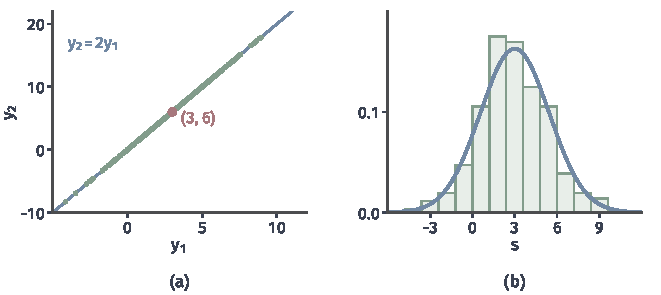
\includegraphics[width=112mm]{figures/07-probability/01-elementary-probability/matplotlib/mvd-gauss-degenerate/figure.pdf}
  \caption{退化高斯分布。(a)$\bm{Y}=(S,2S)^{\top}$的$300$个样本（绿，种子$5$），$S=X_1+X_2$；全部落在直线$y_2=2y_1$（蓝）上，红点为均值$(3,6)$。(b)沿直线的坐标$S$的直方图（浅绿）与$\mathcal{N}(3,6)$密度（蓝）。}
  \label{fig:mvd-gauss-degenerate}
\end{BookInlineFigure}

\paragraph{怎样判断联合高斯}
由式~\eqref{eq:mvd-gaussian-affine}，联合高斯向量的每个分量、每个线性组合$\bm{a}^{\top}\bm{X}$都服从一元高斯分布（方差可能为$0$）。反过来也成立：若对每个$\bm{a}\in\mathbb{R}^{d}$，$\bm{a}^{\top}\bm{X}$都服从一元高斯分布，则$\bm{X}$联合高斯。这个方向本章不证，证明要用到“特征函数唯一确定分布”，特征函数在第~\ref{chap:weak-convergence-of-distributions}章建立。它说明联合高斯是关于所有方向的条件，不是只关于坐标方向的条件。

只检查坐标方向是不够的。设$Z\sim\mathcal{N}(0,1)$，$S$以各$1/2$的概率取$\pm1$，与$Z$独立，考虑$(Z,SZ)$。第二个分量也服从$\mathcal{N}(0,1)$：
\[
 \mathbb{P}(SZ\leq t)=\tfrac12\mathbb{P}(Z\leq t)+\tfrac12\mathbb{P}(-Z\leq t)=\mathbb{P}(Z\leq t) ,
\]
这里用了$-Z$与$Z$同分布。两个分量都是标准高斯。

可是线性组合$Z+SZ$在$S=-1$时恒为$0$，所以$\mathbb{P}(Z+SZ=0)=1/2$。方差为正的一元高斯分布在单点上的概率为$0$，方差为$0$的又只取一个值，$Z+SZ$两样都不是，因而$(Z,SZ)$不是联合高斯。图~\ref{fig:mvd-random-sign}(a)中它的样本只落在两条对角线上，(b)中和的分布有一个质量为$1/2$的原子。

\begin{BookInlineFigure}
  \centering
  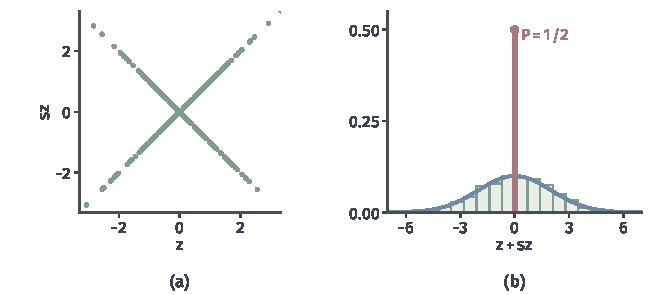
\includegraphics[width=112mm]{figures/07-probability/01-elementary-probability/matplotlib/mvd-random-sign/figure.pdf}
  \caption{分量各自高斯但不联合高斯。(a)$(Z,SZ)$的$400$个样本（绿，种子$3$），$S=\pm1$等可能且与$Z$独立；点只落在两条对角线上。(b)$Z+SZ$的分布：$0$处有概率$1/2$的原子（红），其余部分的密度为$\tfrac12$倍$\mathcal{N}(0,4)$密度（蓝），绿色直方图来自$4000$个模拟值。}
  \label{fig:mvd-random-sign}
\end{BookInlineFigure}

\subsection{条件分布与正交分解}
\label{sec:mvd-gaussian-conditional}

观测到第一台传感器的读数以后，第二台读数的分布变成什么？更一般地，把$\bm{X}$的分量分成两组，观测其中一组，另一组的条件分布是什么？两组什么时候相互独立？为此把$\bm{X}$与参数按相同方式分块：
\[
 \bm{X}=\begin{bmatrix}\bm{X}_a\\\bm{X}_b\end{bmatrix},\qquad
 \bm{\mu}=\begin{bmatrix}\bm{\mu}_a\\\bm{\mu}_b\end{bmatrix},\qquad
 \bm{\Sigma}=\begin{bmatrix}\bm{\Sigma}_{aa}&\bm{\Sigma}_{ab}\\\bm{\Sigma}_{ba}&\bm{\Sigma}_{bb}\end{bmatrix} ,
\]
其中交叉协方差$\bm{\Sigma}_{ab}$就是$\operatorname{Cov}(\bm{X}_a,\bm{X}_b)$，且$\bm{\Sigma}_{ba}=\bm{\Sigma}_{ab}^{\top}$。两组的边缘分布只用到对角块，两组之间的联系全部记在$\bm{\Sigma}_{ab}$里。

\paragraph{零交叉协方差推出独立}
第~\ref{chap:random-vectors}章说明，独立推出不相关，反过来一般不成立。联合高斯是一个重要的例外。

\begin{theorem}[联合高斯的分块独立]
\label{thm:mvd-gaussian-independence}
设$\bm{X}\sim\mathcal{N}(\bm{\mu},\bm{\Sigma})$按上述方式分块。若$\bm{\Sigma}_{ab}=\bm{0}$，则$\bm{X}_a$与$\bm{X}_b$相互独立。
\end{theorem}

\begin{proof}
取矩阵$\bm{A}_a$、$\bm{A}_b$使$\bm{A}_a\bm{A}_a^{\top}=\bm{\Sigma}_{aa}$，$\bm{A}_b\bm{A}_b^{\top}=\bm{\Sigma}_{bb}$，列数分别为$k_a$、$k_b$，再令
\[
 \bm{A}=\begin{bmatrix}\bm{A}_a&\bm{0}\\\bm{0}&\bm{A}_b\end{bmatrix} .
\]
因为$\bm{\Sigma}_{ab}=\bm{0}$，有$\bm{A}\bm{A}^{\top}=\bm{\Sigma}$。由定理~\ref{thm:mvd-gaussian-well-defined}，$\bm{X}$与$\bm{\mu}+\bm{A}\bm{Z}$同分布。把$\bm{Z}$分成前$k_a$个分量$\bm{Z}'$与后$k_b$个分量$\bm{Z}''$，就有
\[
 \bm{X}_a\overset{\mathrm{d}}{=}\bm{\mu}_a+\bm{A}_a\bm{Z}',\qquad \bm{X}_b\overset{\mathrm{d}}{=}\bm{\mu}_b+\bm{A}_b\bm{Z}'' ,
\]
这里$\overset{\mathrm{d}}{=}$表示两组同时同分布。

$\bm{Z}'$与$\bm{Z}''$由不同的独立分量组成，联合密度是两部分密度之积，因而相互独立。对区域$S$、$T$，记$S'$、$T''$为它们在两个仿射映射下的原像，于是
\[
 \mathbb{P}(\bm{X}_a\in S,\ \bm{X}_b\in T)=\mathbb{P}(\bm{Z}'\in S',\ \bm{Z}''\in T'')=\mathbb{P}(\bm{Z}'\in S')\,\mathbb{P}(\bm{Z}''\in T'') .
\]
右边两个因子分别是$\mathbb{P}(\bm{X}_a\in S)$与$\mathbb{P}(\bm{X}_b\in T)$。
\end{proof}

证明没有用到密度，所以$\bm{\Sigma}$奇异时同样成立。逐个分量应用：联合高斯向量的协方差矩阵若是对角的，各分量相互独立。

定理的前提是整个向量联合高斯。上一小节的$(Z,SZ)$中，
\[
 \operatorname{Cov}(Z,SZ)=\mathbb{E}[S]\,\mathbb{E}[Z^{2}]=0 ,
\]
两个分量不相关，也都是标准高斯，却不独立：$\lvert SZ\rvert=\lvert Z\rvert$，知道$Z$以后，$SZ$只剩$\pm Z$两种可能。定理不适用，正是因为它们不联合高斯。

\paragraph{配方求条件分布}
设$\bm{\Sigma}$正定，于是对角块$\bm{\Sigma}_{bb}$也正定，可逆。目标是把联合密度写成“$\bm{x}_b$的边缘密度”乘以“$\bm{x}_a$的某个高斯密度”。关键是对二次型$Q$关于$\bm{x}_a$配方，用矩阵语言就是一步分块消元。令
\[
 \bm{K}=\bm{\Sigma}_{ab}\bm{\Sigma}_{bb}^{-1},\qquad
 \bm{S}=\bm{\Sigma}_{aa}-\bm{\Sigma}_{ab}\bm{\Sigma}_{bb}^{-1}\bm{\Sigma}_{ba},\qquad
 \bm{E}=\begin{bmatrix}\bm{I}&-\bm{K}\\\bm{0}&\bm{I}\end{bmatrix} .
\]
$\bm{S}$是$\bm{\Sigma}$中块$\bm{\Sigma}_{bb}$的Schur补（可参考\BookChapterRef{chap:direct-linear-solvers}{卷二第12章“线性方程的直接求解”}）。

先左乘$\bm{E}$。第一块行的第二块变为$\bm{\Sigma}_{ab}-\bm{K}\bm{\Sigma}_{bb}=\bm{0}$，
\[
 \bm{E}\bm{\Sigma}=\begin{bmatrix}\bm{S}&\bm{0}\\\bm{\Sigma}_{ba}&\bm{\Sigma}_{bb}\end{bmatrix} .
\]
再右乘$\bm{E}^{\top}$。第二块行的第一块变为$\bm{\Sigma}_{ba}-\bm{\Sigma}_{bb}\bm{K}^{\top}$，由$\bm{\Sigma}_{bb}\bm{K}^{\top}=\bm{\Sigma}_{ba}$，它也是$\bm{0}$，得到
\begin{equation}
 \bm{E}\bm{\Sigma}\bm{E}^{\top}=\begin{bmatrix}\bm{S}&\bm{0}\\\bm{0}&\bm{\Sigma}_{bb}\end{bmatrix} .
 \label{eq:mvd-block-elimination}
\end{equation}

式~\eqref{eq:mvd-block-elimination}给出三件事。$\bm{E}$可逆，所以右边与$\bm{\Sigma}$同为正定，$\bm{S}$正定。$\det\bm{E}=1$，所以行列式按块分解。两边求逆，又得到$\bm{\Sigma}^{-1}$的分解：
\[
 \det\bm{\Sigma}=\det\bm{S}\cdot\det\bm{\Sigma}_{bb},\qquad
 \bm{\Sigma}^{-1}=\bm{E}^{\top}\begin{bmatrix}\bm{S}^{-1}&\bm{0}\\\bm{0}&\bm{\Sigma}_{bb}^{-1}\end{bmatrix}\bm{E} .
\]

把最后一式代入$Q$。记$\bm{u}=\bm{x}-\bm{\mu}$，则$\bm{E}\bm{u}$的两块是$\bm{u}_a-\bm{K}\bm{u}_b$与$\bm{u}_b$，于是
\[
 Q(\bm{x})=(\bm{u}_a-\bm{K}\bm{u}_b)^{\top}\bm{S}^{-1}(\bm{u}_a-\bm{K}\bm{u}_b)+\bm{u}_b^{\top}\bm{\Sigma}_{bb}^{-1}\bm{u}_b .
\]
这就是配方的结果：第一项是$\bm{x}_a$围绕$\bm{\mu}_a+\bm{K}\bm{u}_b$的二次型，第二项只含$\bm{x}_b$。

把配方结果和行列式的分解代入式~\eqref{eq:mvd-gaussian-density}，常数与指数都按两组拆开，联合密度成为两个高斯密度之积：第一个是$\bm{x}_a$的均值为$\bm{\mu}_a+\bm{K}\bm{u}_b$、协方差为$\bm{S}$的密度，第二个是$\mathcal{N}(\bm{\mu}_b,\bm{\Sigma}_{bb})$的密度。后者正是$\bm{X}_b$的边缘密度。除以它，按第~\ref{chap:random-vectors}章条件密度的定义得到下面的定理。

\begin{theorem}[高斯条件分布]
\label{thm:mvd-gaussian-conditional}
设$\bm{\Sigma}$正定，$\bm{X}\sim\mathcal{N}(\bm{\mu},\bm{\Sigma})$按上述方式分块。对每个$\bm{x}_b$，给定$\bm{X}_b=\bm{x}_b$时$\bm{X}_a$的条件分布是高斯分布，条件均值与条件协方差分别为
\begin{align}
 \mathbb{E}[\bm{X}_a\mid\bm{X}_b=\bm{x}_b]&=\bm{\mu}_a+\bm{\Sigma}_{ab}\bm{\Sigma}_{bb}^{-1}(\bm{x}_b-\bm{\mu}_b),
 \label{eq:mvd-gauss-cond-mean}\\
 \operatorname{Cov}(\bm{X}_a\mid\bm{X}_b=\bm{x}_b)&=\bm{\Sigma}_{aa}-\bm{\Sigma}_{ab}\bm{\Sigma}_{bb}^{-1}\bm{\Sigma}_{ba} .
 \label{eq:mvd-gauss-cond-cov}
\end{align}
\end{theorem}

回到传感器，观测第一台读数$X_1=x_1$，求第二台$X_2$的条件分布。此时$\bm{X}_a=X_2$，$\bm{X}_b=X_1$，各块都是数：$\Sigma_{aa}=\Sigma_{bb}=2$，$\Sigma_{ab}=1$。代入式~\eqref{eq:mvd-gauss-cond-mean}和式~\eqref{eq:mvd-gauss-cond-cov}，
\[
 \mathbb{E}[X_2\mid X_1=x_1]=1+\frac{x_1-2}{2},\qquad \operatorname{Var}(X_2\mid X_1=x_1)=2-\frac{1}{2}=\frac32 .
\]

若第一台读到$x_1=4$，比均值高$2$，则$X_2\mid X_1=4\sim\mathcal{N}(2,3/2)$。观测之前$X_2\sim\mathcal{N}(1,2)$，$\mathbb{P}(X_2>2)=1-\Phi(1/\sqrt2)\approx0.240$，其中$\Phi$是标准高斯分布函数；观测之后，$\mathbb{P}(X_2>2\mid X_1=4)=0.5$。第一台偏高，把对第二台的预测中心从$1$推到$2$，方差从$2$缩到$1.5$。

图~\ref{fig:mvd-gauss-conditional}(a)中，竖直红线$x_1=4$切过等密度椭圆，切片上的密度重新归一化，就是条件密度；黄线是条件均值$m(x_1)=1+(x_1-2)/2$，它穿过每条竖直切片上密度最高的点。(b)比较了观测前后$X_2$的密度。

\begin{BookInlineFigure}
  \centering
  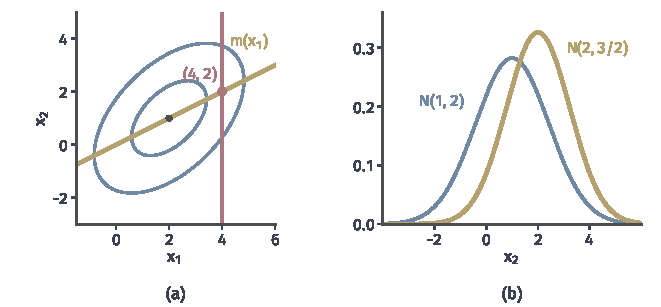
\includegraphics[width=112mm]{figures/07-probability/01-elementary-probability/matplotlib/mvd-gauss-conditional/figure.pdf}
  \caption{传感器例子的条件化。(a)等密度椭圆$Q=1,4$（蓝），观测$x_1=4$（红线），条件均值直线$m(x_1)=1+(x_1-2)/2$（黄），红点$(4,2)$是给定$X_1=4$时$X_2$的条件均值。(b)$X_2$的边缘密度$\mathcal{N}(1,2)$（蓝）与给定$X_1=4$后的条件密度$\mathcal{N}(2,3/2)$（黄）。}
  \label{fig:mvd-gauss-conditional}
\end{BookInlineFigure}

式~\eqref{eq:mvd-gauss-cond-mean}与式~\eqref{eq:mvd-gauss-cond-cov}有两个特点。条件均值是观测值的仿射函数，图中是一条直线。条件协方差完全不依赖观测值：无论第一台读到多少，第二台的剩余不确定性都是$1.5$。一般的联合分布中，条件方差会随条件取值变化，例如三角形区域上的均匀分布，固定的坐标越靠近顶点，另一个坐标可取的范围越窄，条件方差越小。不随观测值变化是高斯模型的特殊性质。

此外，$\bm{\Sigma}_{aa}$与$\bm{S}$之差是半正定矩阵$\bm{\Sigma}_{ab}\bm{\Sigma}_{bb}^{-1}\bm{\Sigma}_{ba}$，所以观测只会减少每个方向上的方差，不会增加。$\bm{\Sigma}_{ab}=\bm{0}$时$\bm{S}=\bm{\Sigma}_{aa}$，条件分布等于边缘分布，与定理~\ref{thm:mvd-gaussian-independence}一致。

\paragraph{正交分解}
条件协方差为什么不随观测值变化？把$\bm{X}_a$减去它的条件均值，看剩下的残差
\[
 \bm{R}=\bm{X}_a-\bm{\mu}_a-\bm{K}(\bm{X}_b-\bm{\mu}_b) .
\]
$(\bm{R},\bm{X}_b)$是$\bm{X}$的仿射像，由式~\eqref{eq:mvd-gaussian-affine}联合高斯。它们的交叉协方差是
\[
 \operatorname{Cov}(\bm{R},\bm{X}_b)=\bm{\Sigma}_{ab}-\bm{K}\bm{\Sigma}_{bb}=\bm{0} .
\]
由定理~\ref{thm:mvd-gaussian-independence}，$\bm{R}$与$\bm{X}_b$独立。

再算残差的协方差。展开后有三项交叉项，每一项都等于$\bm{\Sigma}_{ab}\bm{\Sigma}_{bb}^{-1}\bm{\Sigma}_{ba}$，于是
\[
 \operatorname{Cov}(\bm{R})=\bm{\Sigma}_{aa}-\bm{K}\bm{\Sigma}_{ba}-\bm{\Sigma}_{ab}\bm{K}^{\top}+\bm{K}\bm{\Sigma}_{bb}\bm{K}^{\top}=\bm{S} .
\]
所以$\bm{X}_a$分解成两部分：
\begin{equation}
 \bm{X}_a=\underbrace{\bm{\mu}_a+\bm{K}(\bm{X}_b-\bm{\mu}_b)}_{\text{由}\bm{X}_b\text{决定}}+\underbrace{\bm{R}}_{\text{与}\bm{X}_b\text{独立}},\qquad \bm{R}\sim\mathcal{N}(\bm{0},\bm{S}) .
 \label{eq:mvd-orthogonal-decomposition}
\end{equation}

观测$\bm{X}_b=\bm{x}_b$只确定了第一部分，残差的分布不受影响，所以条件分布是把$\mathcal{N}(\bm{0},\bm{S})$平移到条件均值处。$\bm{K}$的选择恰好使残差与$\bm{X}_b$不相关；用协方差作内积，第一部分就是$\bm{X}_a$在“$\bm{X}_b$的仿射函数”上的正交投影。对联合高斯，不相关又等于独立，于是投影之外不再剩下任何与$\bm{X}_b$有关的东西。

传感器例子中，$X_2$的残差是
\[
 R=X_2-1-\frac{X_1-2}{2}=-\frac12Z_1+\frac12Z_2+Z_3 .
\]
它与$X_1=2+Z_1+Z_2$的协方差是$-\tfrac12+\tfrac12=0$：$Z_1$与$Z_2$的贡献恰好抵消。方差为$\tfrac14+\tfrac14+1=\tfrac32$，与式~\eqref{eq:mvd-gauss-cond-cov}一致。

正交分解的论证只用到$\bm{\Sigma}_{bb}$可逆，不需要整个$\bm{\Sigma}$正定。$\bm{S}$奇异时$\bm{X}$没有联合密度，第~\ref{chap:random-vectors}章的密度比无法直接使用，但式~\eqref{eq:mvd-orthogonal-decomposition}仍说明，给定$\bm{X}_b=\bm{x}_b$后$\bm{X}_a$应当服从$\mathcal{N}(\bm{\mu}_a+\bm{K}(\bm{x}_b-\bm{\mu}_b),\bm{S})$，这是一个退化高斯分布。对零概率条件的严格表述在第~\ref{chap:conditional-distributions}章给出。

\paragraph{观测块退化}
若$\bm{\Sigma}_{bb}$也奇异，观测的各分量之间有线性约束，观测值只能落在$\bm{\mu}_b$加上$\bm{\Sigma}_{bb}$列空间的仿射子空间里，此外的观测值不可能出现。例如增加第三台传感器，它只是第一台的复制品，$X_3=X_1$。观测$(X_1,X_3)=(4,4)$与只观测$X_1=4$含有相同的信息，而$(4,5)$根本不会出现。处理办法是先限制到有效支撑：去掉冗余的分量，只对一组线性无关的观测条件化。

不挑选分量也可以，把$\bm{\Sigma}_{bb}^{-1}$换成Moore--Penrose伪逆$\bm{\Sigma}_{bb}^{+}$（可参考\BookChapterRef{chap:linear-solution-selection}{卷二第11章“线性方程与最小二乘的选解”}），令$\bm{K}=\bm{\Sigma}_{ab}\bm{\Sigma}_{bb}^{+}$。正交分解仍然成立，只需验证$\bm{K}\bm{\Sigma}_{bb}=\bm{\Sigma}_{ab}$。

验证分两步。若$\bm{\Sigma}_{bb}\bm{v}=\bm{0}$，则$\bm{v}^{\top}\bm{X}_b$方差为$0$，恒为常数，它与$\bm{X}_a$的协方差$\bm{\Sigma}_{ab}\bm{v}$为$\bm{0}$；所以$\bm{\Sigma}_{bb}$的零空间含于$\bm{\Sigma}_{ab}$的零空间。又$\bm{I}-\bm{\Sigma}_{bb}^{+}\bm{\Sigma}_{bb}$是到$\bm{\Sigma}_{bb}$零空间的正交投影，于是
\[
 \bm{\Sigma}_{ab}-\bm{K}\bm{\Sigma}_{bb}=\bm{\Sigma}_{ab}\bigl(\bm{I}-\bm{\Sigma}_{bb}^{+}\bm{\Sigma}_{bb}\bigr)=\bm{0} .
\]
此后的论证与前面相同。

\paragraph{样本平均与残差}
正交分解在高斯样本上有一个重要推论。设$X_1,\ldots,X_n$独立同分布于$\mathcal{N}(\mu,\sigma^{2})$，$\sigma>0$，排成向量$\bm{X}=\mu\bm{1}+\sigma\bm{Z}$，于是$\bm{X}\sim\mathcal{N}(\mu\bm{1},\sigma^{2}\bm{I}_n)$。考虑样本平均与残差向量
\[
 \bar{X}_n=\frac1n\bm{1}^{\top}\bm{X},\qquad \bm{R}=\bm{X}-\bar{X}_n\bm{1}=\bm{P}\bm{X},\qquad \bm{P}=\bm{I}_n-\frac1n\bm{1}\bm{1}^{\top} .
\]

几何上，$\bar{X}_n\bm{1}$是$\bm{X}$在直线$\{c\bm{1}\}$上的正交投影，$\bm{R}$是垂直于这条直线的部分。例如观测值$\bm{x}=(1,2,6)^{\top}$，平均为$3$，
\[
 \bm{x}=(3,3,3)^{\top}+(-2,-1,3)^{\top},
\]
第二个向量各分量之和为$0$，与$\bm{1}$正交，图~\ref{fig:mvd-mean-residual}。

\begin{BookInlineFigure}
  \centering
  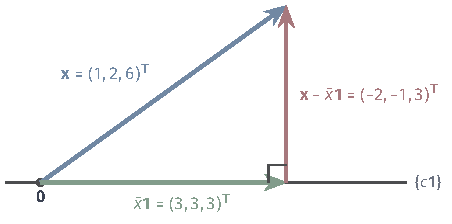
\includegraphics[width=77mm]{figures/07-probability/01-elementary-probability/tikz/mvd-mean-residual/figure.pdf}
  \caption{观测向量$\bm{x}=(1,2,6)^{\top}$（蓝）的正交分解，画在$\bm{1}$与$\bm{x}$张成的平面内并按比例绘制。绿色箭头是在直线$\{c\bm{1}\}$上的投影$\bar{x}\bm{1}$，红色箭头是残差$\bm{x}-\bar{x}\bm{1}$，两者垂直。}
  \label{fig:mvd-mean-residual}
\end{BookInlineFigure}

$(\bar{X}_n,\bm{R})$是$\bm{X}$的线性像，联合高斯。交叉协方差为
\[
 \operatorname{Cov}(\bm{R},\bar{X}_n)=\bm{P}\,(\sigma^{2}\bm{I}_n)\,\frac1n\bm{1}=\frac{\sigma^{2}}{n}\bm{P}\bm{1}=\bm{0} ,
\]
因为$\bm{P}\bm{1}=\bm{1}-\bm{1}=\bm{0}$。由定理~\ref{thm:mvd-gaussian-independence}，$\bar{X}_n$与整个残差向量独立，因而与残差平方和$\lVert\bm{R}\rVert_2^{2}$独立。

两部分的分布也能读出来。$\bar{X}_n\sim\mathcal{N}(\mu,\sigma^{2}/n)$。$\bm{R}\sim\mathcal{N}(\bm{0},\sigma^{2}\bm{P})$，$\bm{P}$是到$n-1$维子空间的正交投影，秩为$n-1$，所以$\bm{R}$是一个退化高斯向量，只在分量和为$0$的超平面上取值。

残差平方和的分布可以用旋转不变性求出。取正交矩阵$\bm{Q}$，其第一行为$\bm{1}^{\top}/\sqrt n$，令$\bm{Y}=\bm{Q}\bm{Z}$，由引理~\ref{lem:mvd-rotation}它仍是标准高斯向量，且$Y_1=\sqrt n\,\bar{Z}$，$\lVert\bm{Y}\rVert_2=\lVert\bm{Z}\rVert_2$。于是
\[
 \sum_{i=1}^{n}(Z_i-\bar{Z})^{2}=\lVert\bm{Z}\rVert_2^{2}-n\bar{Z}^{2}=\sum_{i=2}^{n}Y_i^{2} .
\]
右边是$n-1$个独立标准高斯变量的平方和，服从$\chi^2_{n-1}$（第~\ref{chap:random-variable-transformations}章），所以$\sum_i(X_i-\bar{X}_n)^{2}/\sigma^{2}\sim\chi^2_{n-1}$。样本平均与样本方差独立，是高斯模型统计推断的出发点，可参考\BookChapterRef{chap:parametric-statistical-inference}{卷八第1章“参数化统计推断”}。

这个独立性依赖联合高斯，不是样本平均与残差的一般性质。对任何有限方差的独立同分布样本，$\operatorname{Cov}(\bm{R},\bar{X}_n)=\bm{0}$都成立，但不相关推不出独立。图~\ref{fig:mvd-mean-variance}对比两种总体：高斯样本的平均与残差平方和看不出关系，指数样本的平均越大，残差平方和越分散。

\begin{BookInlineFigure}
  \centering
  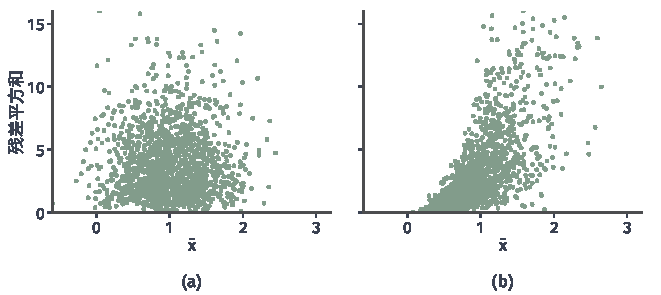
\includegraphics[width=112mm]{figures/07-probability/01-elementary-probability/matplotlib/mvd-mean-variance/figure.pdf}
  \caption{样本平均与残差平方和，每组$n=5$个观测，重复$1500$组。(a)$\mathcal{N}(1,1)$样本（种子$21$），两者的样本相关系数约为$0.02$。(b)$\operatorname{Exp}(1)$样本（均值与方差同为$1$，种子$22$），样本相关系数约为$0.68$，平均越大残差平方和越大。}
  \label{fig:mvd-mean-variance}
\end{BookInlineFigure}


\section{多元t分布}
\label{sec:mvd-t}

多元高斯的尾部很轻：传感器例子中，读数偏离均值超过三个标准差的机会只有千分之几。可是实际环境有时整体变得嘈杂，比如房间的空调启动，两台传感器的误差同时放大。这种“整体波动”不是加在某一台上的独立扰动，而是一个乘在所有分量上的共同尺度。

把多元高斯中固定的尺度换成随机的共同尺度，就得到多元t分布。本节先构造它并求出联合密度，再弄清位置、尺度矩阵和自由度三种参数的不同作用，最后说明共同尺度造成的依赖：即使尺度矩阵是对角的，分量也不独立。

一元情形已在第~\ref{chap:common-distributions}章出现：位置为$\mu$、尺度为$s>0$、自由度为$\nu>0$的t分布密度是
\[
 f(x)=\frac{\Gamma\bigl(\frac{\nu+1}{2}\bigr)}{\Gamma\bigl(\frac{\nu}{2}\bigr)\sqrt{\nu\pi}\,s}\Bigl(1+\frac{(x-\mu)^{2}}{\nu s^{2}}\Bigr)^{-(\nu+1)/2} ,
\]
$\nu=1$时就是Cauchy分布。下面的构造在$d=1$时回到它。

\subsection{正态尺度混合}
\label{sec:mvd-t-mixture}

\paragraph{构造}
取一个高斯向量和一个控制尺度的正随机变量，两者独立，用后者统一放大前者。为使结果的边缘回到一元t分布，尺度取为$\chi^2$变量倒数的平方根。

\begin{definition}[多元t分布]
\label{def:mvd-t}
设$\nu>0$，$\bm{\mu}\in\mathbb{R}^{d}$，$\bm{\Sigma}$是$d\times d$正定矩阵。$\bm{Z}\sim\mathcal{N}(\bm{0},\bm{\Sigma})$与$U\sim\chi^2_\nu$相互独立，令
\begin{equation}
 \bm{X}=\bm{\mu}+\sqrt{\nu/U}\,\bm{Z} .
 \label{eq:mvd-t-construction}
\end{equation}
称$\bm{X}$服从位置为$\bm{\mu}$、\term{尺度矩阵}（scale matrix）为$\bm{\Sigma}$、自由度为$\nu$的\term{多元t分布}（multivariate t distribution）。
\end{definition}

记$V=\sqrt{\nu/U}$。它对所有分量相同：$\bm{X}-\bm{\mu}=V\bm{Z}$的每个分量都乘以同一个$V$。这种把高斯向量乘上一个独立随机尺度的构造称为\term{正态尺度混合}（normal scale mixture）：固定$U=u$，$\bm{X}=\bm{\mu}+\sqrt{\nu/u}\,\bm{Z}$，由式~\eqref{eq:mvd-gaussian-affine}，
\[
 \bm{X}\text{在}U=u\text{时服从}\ \mathcal{N}\Bigl(\bm{\mu},\ \frac{\nu}{u}\bm{\Sigma}\Bigr) .
\]
$\bm{X}$的分布就是这些高斯分布按$U$的分布加权混合。

$U$的均值是$\nu$，所以$V$大致在$1$附近，但$U$可以很接近$0$，此时$V$很大，整个向量被大幅放大。图~\ref{fig:mvd-t-scale}(a)画出不同自由度下$V$的密度：$\nu=1$时$V$有很长的右尾，$\nu=30$时$V$已经紧紧围着$1$。

\paragraph{联合密度}
因为$\bm{Z}$与$U$独立，$(\bm{Z},U)$的联合密度是两者密度之积。对区域$S$，先对$\bm{z}$积分、再对$u$积分，
\[
 \mathbb{P}(\bm{X}\in S)=\int_0^{\infty}f_U(u)\,\mathbb{P}\Bigl(\bm{\mu}+\sqrt{\nu/u}\,\bm{Z}\in S\Bigr)\,\mathrm{d}u .
\]
括号里的概率是$\mathcal{N}(\bm{\mu},(\nu/u)\bm{\Sigma})$的密度在$S$上的积分。被积函数非负，可以交换两次积分的次序，于是$\bm{X}$有密度
\begin{equation}
 f_{\bm{X}}(\bm{x})=\int_0^{\infty}f_U(u)\,g_u(\bm{x})\,\mathrm{d}u ,
 \label{eq:mvd-scale-mixture-density}
\end{equation}
其中$g_u$是$\mathcal{N}(\bm{\mu},(\nu/u)\bm{\Sigma})$的密度。式~\eqref{eq:mvd-scale-mixture-density}对任何独立的正尺度都成立，下一节的多元Laplace分布也用它。

\begin{theorem}[多元t密度]
\label{thm:mvd-t-density}
定义~\ref{def:mvd-t}中的$\bm{X}$有联合密度
\begin{equation}
 f_{\bm{X}}(\bm{x})=\frac{\Gamma\bigl(\frac{\nu+d}{2}\bigr)}{\Gamma\bigl(\frac{\nu}{2}\bigr)(\nu\pi)^{d/2}(\det\bm{\Sigma})^{1/2}}\Bigl(1+\frac{Q(\bm{x})}{\nu}\Bigr)^{-(\nu+d)/2},
 \label{eq:mvd-t-density}
\end{equation}
其中$Q$由式~\eqref{eq:mvd-gaussian-quadratic}给出。
\end{theorem}

\begin{proof}
把$\bm{\Sigma}$换成$(\nu/u)\bm{\Sigma}$，式~\eqref{eq:mvd-gaussian-density}给出
\[
 g_u(\bm{x})=\frac{u^{d/2}}{(2\pi\nu)^{d/2}(\det\bm{\Sigma})^{1/2}}\exp\Bigl(-\frac{uQ}{2\nu}\Bigr) .
\]
$\chi^2_\nu=\operatorname{Gamma}(\nu/2,1/2)$，其密度为
\[
 f_U(u)=\frac{u^{\nu/2-1}\mathrm{e}^{-u/2}}{2^{\nu/2}\Gamma(\nu/2)},\qquad u>0 .
\]

两者相乘，$u$的幂次合并为$u^{(\nu+d)/2-1}$，指数合并为$-u(1+Q/\nu)/2$。由Gamma积分
\[
 \int_0^{\infty}u^{a-1}\mathrm{e}^{-bu}\,\mathrm{d}u=\Gamma(a)\,b^{-a},\qquad a,b>0,
\]
取$a=(\nu+d)/2$，$b=(1+Q/\nu)/2$，
\[
 \int_0^{\infty}u^{\frac{\nu+d}{2}-1}\mathrm{e}^{-\frac{u}{2}(1+Q/\nu)}\,\mathrm{d}u=\Gamma\Bigl(\frac{\nu+d}{2}\Bigr)\,2^{(\nu+d)/2}\Bigl(1+\frac{Q}{\nu}\Bigr)^{-(\nu+d)/2} .
\]
最后整理常数：$2^{(\nu+d)/2}$与$f_U$中的$2^{-\nu/2}$合成$2^{d/2}$，再与$(2\pi\nu)^{-d/2}$合成$(\nu\pi)^{-d/2}$。
\end{proof}

$d=1$、$\bm{\Sigma}=s^{2}$时，$Q=(x-\mu)^{2}/s^{2}$，式~\eqref{eq:mvd-t-density}就是本节开头的一元t密度。与高斯一样，密度只通过$Q$依赖$\bm{x}$，等密度面仍是以$\bm{\mu}$为中心、由$\bm{\Sigma}$决定形状的椭球；这类分布称为\term{椭圆分布}（elliptical distribution）。不同的是密度沿椭球向外的衰减方式：高斯是$\mathrm{e}^{-Q/2}$，t是$Q$的负幂。

取$d=2$、$\nu=5$、$\bm{\mu}=\bm{0}$、$\bm{\Sigma}=\bm{I}$，由$\Gamma(3.5)=2.5\,\Gamma(2.5)$，常数是
\[
 \frac{\Gamma(3.5)}{\Gamma(2.5)\cdot5\pi}=\frac{2.5}{5\pi}=\frac{1}{2\pi},
\]
中心密度恰好与二维标准高斯相同。在$Q=25$，也就是离中心$5$个单位处，两者分别是
\[
 \frac{1}{2\pi}\Bigl(1+\frac{25}{5}\Bigr)^{-7/2}\approx3.0\times10^{-4},\qquad \frac{1}{2\pi}\mathrm{e}^{-25/2}\approx5.9\times10^{-7} ,
\]
相差约$500$倍。

\begin{BookInlineFigure}
  \centering
  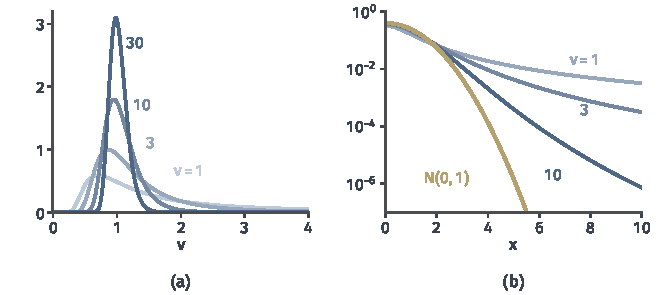
\includegraphics[width=112mm]{figures/07-probability/01-elementary-probability/matplotlib/mvd-t-scale/figure.pdf}
  \caption{共同尺度与尾部。(a)共同尺度$V=\sqrt{\nu/U}$的密度，$\nu=1,3,10,30$（蓝色由浅到深）；自由度越大，$V$越集中在$1$附近。(b)一个分量（$\Sigma_{i,i}=1$）的密度，纵轴取对数：t分布$\nu=1,3,10$（蓝色由浅到深）与$\mathcal{N}(0,1)$（黄）。}
  \label{fig:mvd-t-scale}
\end{BookInlineFigure}

\subsection{参数与矩}
\label{sec:mvd-t-moments}

\paragraph{位置与均值}
由构造，$\bm{X}-\bm{\mu}=V\bm{Z}$关于$\bm{\mu}$对称：$V\bm{Z}$与$-V\bm{Z}$同分布。所以$\bm{\mu}$总是分布的对称中心，也是每个分量的中位数。它是不是均值，要看$\bm{X}$的分量是否可积。

由$V$与$\bm{Z}$独立，
\[
 \mathbb{E}\lvert X_i-\mu_i\rvert=\mathbb{E}[V]\,\mathbb{E}\lvert Z_i\rvert ,
\]
而$\mathbb{E}\lvert Z_i\rvert$有限且为正。对$V$的矩，设$k\geq0$，由$U$的密度，
\[
 \mathbb{E}\bigl[U^{-k/2}\bigr]=\int_0^{\infty}\frac{u^{\nu/2-k/2-1}\mathrm{e}^{-u/2}}{2^{\nu/2}\Gamma(\nu/2)}\,\mathrm{d}u
\]
的有限性只取决于原点附近：积分在$0$附近收敛当且仅当$\nu/2-k/2>0$。

所以$\mathbb{E}[V^{k}]=\nu^{k/2}\mathbb{E}[U^{-k/2}]$在$k<\nu$时有限，在$k\geq\nu$时为无穷，从而
\[
 \mathbb{E}\lvert X_i-\mu_i\rvert^{k}<\infty\quad\Longleftrightarrow\quad k<\nu .
\]
特别地，$\nu>1$时均值存在，由$\mathbb{E}[\bm{Z}]=\bm{0}$，均值等于$\bm{\mu}$；$\nu\leq1$时均值不存在，$\bm{\mu}$只是位置。Cauchy情形$\nu=1$就是这样。

\paragraph{尺度矩阵与协方差}
$k=2$时，算出Gamma积分得
\[
 \mathbb{E}[1/U]=\frac{\Gamma(\nu/2-1)}{2\Gamma(\nu/2)}=\frac{1}{\nu-2},\qquad \nu>2 .
\]
于是$\nu>2$时
\begin{equation}
 \operatorname{Cov}(\bm{X})=\mathbb{E}[V^{2}]\,\operatorname{Cov}(\bm{Z})=\frac{\nu}{\nu-2}\,\bm{\Sigma} .
 \label{eq:mvd-t-cov}
\end{equation}
所以$\bm{\Sigma}$不是协方差矩阵，而是尺度矩阵：它决定椭球的形状和方向，协方差还要乘以共同尺度的二阶矩。两者只差一个正数倍，相关系数矩阵相同。

各种矩的存在条件按自由度列在表~\ref{tab:mvd-t-moments}中。

\begin{BookInlineTable}
  \centering
  \begin{tabular}{lcccc}
    \toprule
    自由度 & $0<\nu\leq1$ & $1<\nu\leq2$ & $2<\nu\leq4$ & $\nu>4$\\
    \midrule
    均值$\bm{\mu}$ & 不存在 & 存在 & 存在 & 存在\\
    协方差 & 不存在 & 不存在 & $\frac{\nu}{\nu-2}\bm{\Sigma}$ & $\frac{\nu}{\nu-2}\bm{\Sigma}$\\
    四阶矩 & 不存在 & 不存在 & 不存在 & 存在\\
    \bottomrule
  \end{tabular}
  \caption{多元t分布各阶矩的存在条件，“存在”指对应的期望有限。}
  \label{tab:mvd-t-moments}
\end{BookInlineTable}

\paragraph{边缘与线性组合}
取出第$i$个分量，$X_i=\mu_i+VZ_i$，$Z_i\sim\mathcal{N}(0,\Sigma_{i,i})$，$V$不变。这正是$d=1$时的同一构造，所以$X_i$服从位置$\mu_i$、尺度$\sqrt{\Sigma_{i,i}}$、自由度$\nu$的一元t分布。同理，$\bm{a}^{\top}\bm{X}$等于$\bm{a}^{\top}\bm{\mu}$加上$V\,\bm{a}^{\top}\bm{Z}$，服从尺度为$\sqrt{\bm{a}^{\top}\bm{\Sigma}\bm{a}}$的一元t分布，任意一组分量服从相应子矩阵的多元t分布。边缘与整体的自由度相同，因为它们共用同一个$U$。

一元t密度的尾部按$\lvert x\rvert^{-(\nu+1)}$衰减，所以$\nu$越小尾部越重，图~\ref{fig:mvd-t-scale}(b)。由上面的矩条件，这与“$k\geq\nu$阶矩不存在”是一回事：尾部太重，高阶矩积不出来。

\paragraph{自由度增大时}
$U\sim\chi^2_\nu$的均值为$\nu$、方差为$2\nu$，所以$U/\nu$的均值为$1$、方差为$2/\nu$。由第~\ref{chap:tail-probabilities}章的Chebyshev不等式，对任意$\varepsilon>0$，
\[
 \mathbb{P}\Bigl(\Bigl\lvert\frac{U}{\nu}-1\Bigr\rvert\geq\varepsilon\Bigr)\leq\frac{2}{\nu\varepsilon^{2}} .
\]
$\nu\to\infty$时右边趋于$0$，共同尺度$V=(U/\nu)^{-1/2}$越来越确定地接近$1$，$\bm{X}$也就越来越像$\mathcal{N}(\bm{\mu},\bm{\Sigma})$。从密度看，$(1+Q/\nu)^{-(\nu+d)/2}\to\mathrm{e}^{-Q/2}$，常数也趋于高斯的常数。$\nu$因此度量了“尺度有多不确定”：自由度小，尺度波动大，尾部重；自由度大，模型退回高斯。

\subsection{分量的依赖}
\label{sec:mvd-t-dependence}

设$\bm{\Sigma}$是对角矩阵，为简单起见取$\bm{\mu}=\bm{0}$、$\bm{\Sigma}=\bm{I}_d$。固定$U=u$时，$\bm{X}\sim\mathcal{N}(\bm{0},(\nu/u)\bm{I}_d)$，各分量相互独立：给定共同尺度，分量条件独立。$\nu>2$时由式~\eqref{eq:mvd-t-cov}，协方差矩阵也是对角的，分量两两不相关。可是不知道$U$的时候，一个分量很大，说明共同尺度可能很大，另一个分量也就更可能大。

\paragraph{联合密度不能分解}
先证明，对任何$\nu>0$，$d=2$时$X_1$与$X_2$不独立。若两者独立，对以$(x_1,x_2)$为中心、边长为$h$的小正方形，联合概率等于两个边长为$h$的区间概率之积。两边除以$h^{2}$，令$h\to0$，由三个密度的连续性得到
\[
 f_{\bm{X}}(x_1,x_2)=f_{X_1}(x_1)\,f_{X_2}(x_2)\qquad\text{对一切}(x_1,x_2) .
\]
于是对任意$a,b$，必须有
\[
 f_{\bm{X}}(a,b)\,f_{\bm{X}}(0,0)=f_{\bm{X}}(a,0)\,f_{\bm{X}}(0,b) ,
\]
因为两边都等于同样四个边缘密度值之积。

取$a=b=1$检验。由式~\eqref{eq:mvd-t-density}，$f_{\bm{X}}$与$k(Q)=(1+Q/\nu)^{-(\nu+2)/2}$成正比，上式要求$k(2)k(0)=k(1)^{2}$。但
\[
 \Bigl(1+\frac1\nu\Bigr)^{2}=1+\frac2\nu+\frac{1}{\nu^{2}}>1+\frac2\nu ,
\]
两边取$-(\nu+2)/2$次幂，不等号反向，得到$k(1)^{2}<k(2)=k(2)k(0)$。等式不成立，所以$X_1$与$X_2$不独立。

\paragraph{条件方差随观测增大}
依赖的方式可以算得很具体。固定$X_1=x_1$，把联合密度看成$x_2$的函数并提出与$x_2$无关的因子：
\[
 \Bigl(1+\frac{x_1^{2}+x_2^{2}}{\nu}\Bigr)^{-\frac{\nu+2}{2}}=\Bigl(1+\frac{x_1^{2}}{\nu}\Bigr)^{-\frac{\nu+2}{2}}\Bigl(1+\frac{x_2^{2}}{\nu+x_1^{2}}\Bigr)^{-\frac{\nu+2}{2}} .
\]
第二个因子正是自由度$\nu+1$、尺度$s$满足$(\nu+1)s^{2}=\nu+x_1^{2}$的一元t密度的形状。

所以给定$X_1=x_1$，$X_2$服从自由度$\nu+1$、尺度平方为$(\nu+x_1^{2})/(\nu+1)$的t分布。$\nu>1$时它的自由度大于$2$，由式~\eqref{eq:mvd-t-cov}的一元情形，
\begin{equation}
 \mathbb{E}[X_2^{2}\mid X_1=x_1]=\frac{\nu+x_1^{2}}{\nu+1}\cdot\frac{\nu+1}{\nu-1}=\frac{\nu+x_1^{2}}{\nu-1} .
 \label{eq:mvd-t-conditional-second-moment}
\end{equation}
它随$\lvert x_1\rvert$增大而增大。

取$\nu=5$：$X_2$的无条件方差是$5/3\approx1.67$；观测到$x_1=0$时条件二阶矩是$5/4=1.25$，观测到$x_1=3$时变为$14/4=3.5$。第一个分量平静，说明共同尺度多半不大，第二个分量也收敛一些；第一个分量剧烈，第二个分量的波动随之放大。图~\ref{fig:mvd-t-dependence}(b)用模拟样本核对了式~\eqref{eq:mvd-t-conditional-second-moment}。

\begin{BookInlineFigure}
  \centering
  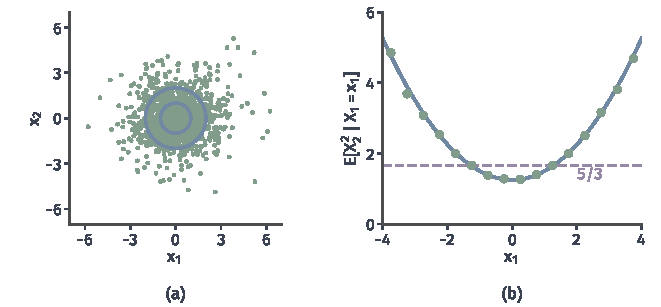
\includegraphics[width=112mm]{figures/07-probability/01-elementary-probability/matplotlib/mvd-t-dependence/figure.pdf}
  \caption{$\nu=5$、$\bm{\Sigma}=\bm{I}$的二维t分布，分量不相关但不独立。(a)$1500$个样本（绿，种子$31$）与等密度圆$Q=1,4$（蓝）；远处的点往往两个坐标同时偏大。(b)条件二阶矩$\mathbb{E}[X_2^{2}\mid X_1=x_1]=(5+x_1^{2})/4$（蓝），绿点是$40$万个样本（种子$32$）按$x_1$分组、组宽$0.5$的组内平均，紫色虚线是无条件方差$5/3$。}
  \label{fig:mvd-t-dependence}
\end{BookInlineFigure}

\paragraph{平方的协方差}
同样的依赖也能从矩看出来。$\nu>4$时$\mathbb{E}[1/U^{2}]=1/((\nu-2)(\nu-4))$，由$V$与$\bm{Z}$独立及$Z_1,Z_2$独立，
\[
 \mathbb{E}[X_1^{2}X_2^{2}]=\mathbb{E}[V^{4}]\,\mathbb{E}[Z_1^{2}]\,\mathbb{E}[Z_2^{2}]=\frac{\nu^{2}}{(\nu-2)(\nu-4)} .
\]
而$\mathbb{E}[X_1^{2}]$与$\mathbb{E}[X_2^{2}]$都等于$\nu/(\nu-2)$，两者之差为
\[
 \operatorname{Cov}(X_1^{2},X_2^{2})=\frac{2\nu^{2}}{(\nu-2)^{2}(\nu-4)}>0 .
\]
$\nu=5$时它等于$50/9\approx5.56$。$X_1$与$X_2$不相关，$X_1^{2}$与$X_2^{2}$却正相关：共同尺度让两个分量的大小一起涨落，而符号仍各自随机，所以线性的协方差看不到这种依赖。

如果想要“边缘是t分布、分量独立”的模型，就应让每个分量各用一个独立的尺度：$X_i=\mu_i+\sqrt{\nu/U_i}\,Z_i$，$U_1,\ldots,U_d$相互独立。它的边缘与多元t相同，协方差也相同，却是另一个联合分布，等密度线不再是椭圆。第~\ref{sec:mvd-comparison}节会比较两种模型在“同时出现大值”上的差别。


\section{多元Laplace分布}
\label{sec:mvd-laplace}

t分布的重尾有代价：自由度小的时候，方差甚至均值都不存在。有些波动比高斯更“尖”、尾部更厚，却仍有全部有限阶矩，一元时第~\ref{chap:common-distributions}章的Laplace分布正适合描述它们。它的密度是$(2b)^{-1}\mathrm{e}^{-\lvert x-\mu\rvert/b}$，尾部按指数衰减，比高斯的$\mathrm{e}^{-x^{2}/2}$慢，但仍快过任何负幂。

推广到多元，答案并不唯一。最直接的做法是让各分量独立地服从一元Laplace分布；另一种做法沿用上一节的思路，用一个共同的随机尺度放大高斯向量。本节采用后者，即由共同指数尺度混合得到的对称椭圆型版本，称为\term{多元Laplace分布}（multivariate Laplace distribution），并在最后与独立分量的乘积模型对照。

\subsection{正态指数混合}
\label{sec:mvd-laplace-mixture}

\paragraph{构造}
上一节的共同尺度$\nu/U$有很长的右尾，这是t分布矩不存在的根源。换一个右尾短的尺度，就能保留混合带来的厚尾，又不丢掉矩。指数分布是最简单的选择。

\begin{definition}[多元Laplace分布]
\label{def:mvd-laplace}
设$\bm{\mu}\in\mathbb{R}^{d}$，$\bm{\Sigma}$是$d\times d$正定矩阵。$W\sim\operatorname{Exp}(1)$（速率为$1$）与$\bm{Z}\sim\mathcal{N}(\bm{0},\bm{\Sigma})$相互独立，令
\begin{equation}
 \bm{X}=\bm{\mu}+\sqrt{W}\,\bm{Z} .
 \label{eq:mvd-laplace-construction}
\end{equation}
称$\bm{X}$服从参数为$\bm{\mu}$、$\bm{\Sigma}$的多元Laplace分布。
\end{definition}

固定$W=w$，$\bm{X}\sim\mathcal{N}(\bm{\mu},w\bm{\Sigma})$，所以这仍是一个正态尺度混合，只是这次混合的是方差因子$W$本身。图~\ref{fig:mvd-mixing-laws}比较两种方差因子：$\nu=5$的t分布用$5/U$，本节用$W$。两者都可以取远大于$1$的值，这是厚尾的来源；但$W$的尾概率是$\mathrm{e}^{-v}$，$5/U$的尾概率只按$v^{-5/2}$下降。

\begin{BookInlineFigure}
  \centering
  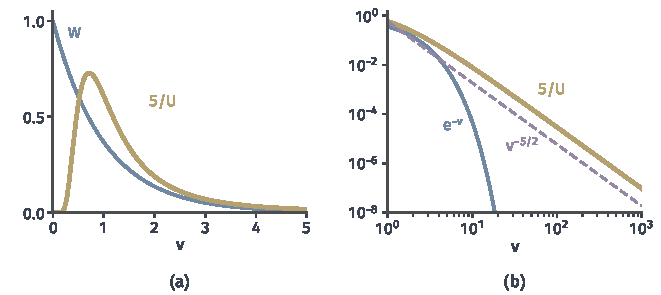
\includegraphics[width=112mm]{figures/07-probability/01-elementary-probability/matplotlib/mvd-mixing-laws/figure.pdf}
  \caption{两种正态尺度混合的方差因子。(a)密度：多元Laplace的$W\sim\operatorname{Exp}(1)$（蓝）与$\nu=5$的多元t的$5/U$，$U\sim\chi^2_5$（黄）。(b)尾概率$\mathbb{P}(\cdot>v)$，双对数坐标；紫色虚线是斜率为$-5/2$的参考线。尾概率由精确密度数值积分得到。}
  \label{fig:mvd-mixing-laws}
\end{BookInlineFigure}

\paragraph{均值、协方差与矩}
$\sqrt W$的均值$\Gamma(3/2)=\sqrt\pi/2$有限，由独立性及$\mathbb{E}[\bm{Z}]=\bm{0}$，$\mathbb{E}[\bm{X}]=\bm{\mu}$。协方差为
\begin{equation}
 \operatorname{Cov}(\bm{X})=\mathbb{E}[W]\,\bm{\Sigma}=\bm{\Sigma} .
 \label{eq:mvd-laplace-cov}
\end{equation}
与t分布不同，这里的$\bm{\Sigma}$就是协方差矩阵。

更高阶的矩同样存在。对任意$k\geq0$，$\mathbb{E}[W^{k/2}]=\Gamma(1+k/2)<\infty$，而高斯分量的各阶矩都有限，所以
\[
 \mathbb{E}\lvert X_i-\mu_i\rvert^{k}=\Gamma\Bigl(1+\frac k2\Bigr)\,\mathbb{E}\lvert Z_i\rvert^{k}<\infty .
\]
这正是选用指数尺度的目的：混合让尾部变厚，指数尺度的短尾又保证一切矩有限。

\paragraph{联合密度}
由式~\eqref{eq:mvd-scale-mixture-density}，把$g_u$换成$\mathcal{N}(\bm{\mu},w\bm{\Sigma})$的密度、$f_U$换成$\mathrm{e}^{-w}$，
\begin{equation}
 f_{\bm{X}}(\bm{x})=\frac{1}{(2\pi)^{d/2}(\det\bm{\Sigma})^{1/2}}\int_0^{\infty}w^{-d/2}\exp\Bigl(-w-\frac{Q(\bm{x})}{2w}\Bigr)\,\mathrm{d}w .
 \label{eq:mvd-laplace-density}
\end{equation}
密度仍只通过$Q(\bm{x})$依赖$\bm{x}$，所以多元Laplace分布也是椭圆分布，等密度面与$\mathcal{N}(\bm{\mu},\bm{\Sigma})$的相同。剩下的问题是沿着椭球向外，密度怎样衰减。下面的积分让我们在$d=1$和$d=3$时算出初等形式。

\begin{lemma}[一个指数积分]
\label{lem:mvd-exp-integral}
对$a>0$，
\begin{equation}
 \begin{aligned}
  \int_0^{\infty}w^{-1/2}\mathrm{e}^{-w-a/w}\,\mathrm{d}w&=\sqrt\pi\,\mathrm{e}^{-2\sqrt a},\\
  \int_0^{\infty}w^{-3/2}\mathrm{e}^{-w-a/w}\,\mathrm{d}w&=\sqrt{\frac{\pi}{a}}\,\mathrm{e}^{-2\sqrt a} .
 \end{aligned}
 \label{eq:mvd-exp-integral}
\end{equation}
\end{lemma}

\begin{proof}
第一个积分中令$w=s^{2}$，$\mathrm{d}w=2s\,\mathrm{d}s$，再记$c=\sqrt a$并在指数中配方，$s^{2}+c^{2}/s^{2}=(s-c/s)^{2}+2c$，于是
\[
 \int_0^{\infty}w^{-1/2}\mathrm{e}^{-w-a/w}\,\mathrm{d}w=2\int_0^{\infty}\mathrm{e}^{-s^{2}-c^{2}/s^{2}}\,\mathrm{d}s=2\mathrm{e}^{-2c}J,
\]
其中
\[
 J=\int_0^{\infty}\mathrm{e}^{-(s-c/s)^{2}}\,\mathrm{d}s .
\]

求$J$用一个对称技巧。令$s=c/t$，$\mathrm{d}s=-c\,t^{-2}\mathrm{d}t$，积分限对调，$(s-c/s)^{2}=(c/t-t)^{2}$，所以
\[
 J=\int_0^{\infty}\mathrm{e}^{-(t-c/t)^{2}}\,\frac{c}{t^{2}}\,\mathrm{d}t .
\]
把两种写法相加，
\[
 2J=\int_0^{\infty}\mathrm{e}^{-(s-c/s)^{2}}\Bigl(1+\frac{c}{s^{2}}\Bigr)\,\mathrm{d}s .
\]
再令$y=s-c/s$，它在$(0,\infty)$上严格递增，从$-\infty$变到$\infty$，且$\mathrm{d}y=(1+c/s^{2})\,\mathrm{d}s$，
\[
 2J=\int_{-\infty}^{\infty}\mathrm{e}^{-y^{2}}\,\mathrm{d}y=\sqrt\pi .
\]
所以$J=\sqrt\pi/2$，第一个等式成立。

第二个积分由第一个换元得到。在第一个积分中令$w=a/t$，$\mathrm{d}w=-a\,t^{-2}\mathrm{d}t$，$w^{-1/2}=t^{1/2}a^{-1/2}$，指数$-w-a/w$变为$-a/t-t$，于是
\[
 \sqrt\pi\,\mathrm{e}^{-2\sqrt a}=\int_0^{\infty}t^{1/2}a^{-1/2}\,\mathrm{e}^{-t-a/t}\,\frac{a}{t^{2}}\,\mathrm{d}t=\sqrt a\int_0^{\infty}t^{-3/2}\mathrm{e}^{-t-a/t}\,\mathrm{d}t .
\]
两边除以$\sqrt a$即得第二个等式。
\end{proof}

$d=1$时$\bm{\Sigma}=\sigma^{2}$，$Q=(x-\mu)^{2}/\sigma^{2}$。式~\eqref{eq:mvd-laplace-density}中取$a=Q/2$，用式~\eqref{eq:mvd-exp-integral}的第一式，$2\sqrt a=\sqrt2\,\lvert x-\mu\rvert/\sigma$，
\[
 f_X(x)=\frac{1}{\sqrt{2\pi}\,\sigma}\sqrt\pi\,\mathrm{e}^{-\sqrt2\lvert x-\mu\rvert/\sigma}=\frac{1}{\sqrt2\,\sigma}\mathrm{e}^{-\sqrt2\lvert x-\mu\rvert/\sigma} .
\]
这正是尺度$b=\sigma/\sqrt2$的一元Laplace密度，其方差$2b^{2}=\sigma^{2}$与式~\eqref{eq:mvd-laplace-cov}一致。

$d=3$时用第二式，同样取$a=Q/2$，常数$(2\pi)^{-3/2}\sqrt{2\pi}=(2\pi)^{-1}$，得到
\[
 f_{\bm{X}}(\bm{x})=\frac{1}{2\pi(\det\bm{\Sigma})^{1/2}}\cdot\frac{\mathrm{e}^{-\sqrt{2Q(\bm{x})}}}{\sqrt{Q(\bm{x})}} .
\]
它不只是$\mathrm{e}^{-\sqrt{2Q}}$：多出的因子$Q^{-1/2}$让密度在中心$\bm{x}=\bm{\mu}$处趋于无穷。

\paragraph{中心的奇性}
$d\geq2$时中心的奇性是普遍的，不依赖初等形式。若$Q(\bm{x})\leq\varepsilon<1$，式~\eqref{eq:mvd-laplace-density}中的积分只保留$w\in[\varepsilon,1]$一段，在这一段上$\mathrm{e}^{-w}\geq\mathrm{e}^{-1}$，$Q/(2w)\leq\tfrac12$，于是
\[
 \int_0^{\infty}w^{-d/2}\mathrm{e}^{-w-Q/(2w)}\,\mathrm{d}w\geq\mathrm{e}^{-3/2}\int_{\varepsilon}^{1}w^{-d/2}\,\mathrm{d}w .
\]
$d\geq2$时右边在$\varepsilon\to0$时趋于无穷，所以$\bm{x}\to\bm{\mu}$时$f_{\bm{X}}(\bm{x})\to\infty$。原因是$W$可以很接近$0$：此时高斯分量被压得很窄，在中心堆出越来越高的尖峰，维数越高，这些尖峰叠加得越陡。

奇性不影响概率的计算，密度仍然可积，总积分为$1$。它提醒我们：多元Laplace的密度沿椭球向外不是简单的$\mathrm{e}^{-\sqrt{2Q}}$，只有$d=1$时才是。把密度直接设成$c\,\mathrm{e}^{-\sqrt{2Q}}$得到的是另一个模型，与本节由共同指数尺度给出的构造不同。图~\ref{fig:mvd-laplace-shape}(b)沿一条射线画出$d=1,2,3$时的密度，$d=2$时的积分不是初等函数，由数值积分得到。

\begin{BookInlineFigure}
  \centering
  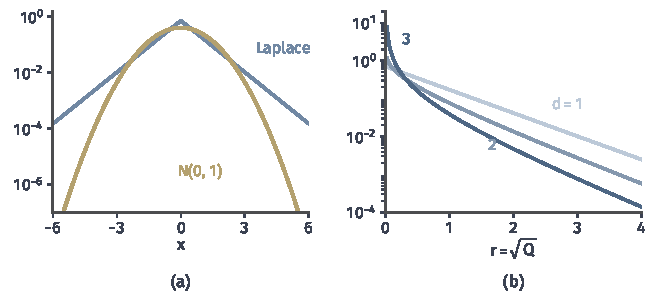
\includegraphics[width=112mm]{figures/07-probability/01-elementary-probability/matplotlib/mvd-laplace-shape/figure.pdf}
  \caption{多元Laplace的形状，$\bm{\mu}=\bm{0}$，$\bm{\Sigma}=\bm{I}_d$，纵轴取对数。(a)一个分量的密度：尺度$b=1/\sqrt2$的Laplace密度（蓝）与方差同为$1$的$\mathcal{N}(0,1)$密度（黄）；Laplace在中心更尖，在远处更厚。(b)沿射线的联合密度随$r=\sqrt Q$的变化，$d=1,2,3$（蓝色由浅到深），由式~\eqref{eq:mvd-laplace-density}数值积分；$d=2,3$时中心处趋于无穷。}
  \label{fig:mvd-laplace-shape}
\end{BookInlineFigure}

\subsection{边缘与共同尺度}
\label{sec:mvd-laplace-marginal}

\paragraph{边缘是一元Laplace}
取出第$i$个分量，$X_i=\mu_i+\sqrt W\,Z_i$，$Z_i\sim\mathcal{N}(0,\Sigma_{i,i})$，$W$不变。这就是$d=1$的构造，由上面的计算，$X_i$服从位置$\mu_i$、尺度
\begin{equation}
 b_i=\sqrt{\Sigma_{i,i}/2}
 \label{eq:mvd-laplace-marginal-scale}
\end{equation}
的一元Laplace分布，尺度的含义与第~\ref{chap:common-distributions}章相同。同理，$\bm{a}^{\top}\bm{X}$服从尺度为$\sqrt{\bm{a}^{\top}\bm{\Sigma}\bm{a}/2}$的一元Laplace分布，任意一组分量服从相应子矩阵的多元Laplace分布。

与同方差的高斯相比，Laplace边缘在中心更尖、远处更厚。图~\ref{fig:mvd-laplace-shape}(a)中两者方差都是$1$：Laplace在$0$处的密度是$1/\sqrt2\approx0.707$，高斯是$0.399$；而$\mathbb{P}(\lvert X_i\rvert>3)$，Laplace为$\mathrm{e}^{-3\sqrt2}\approx0.0144$，高斯约为$0.0027$。

\paragraph{共同尺度造成依赖}
取$\bm{\mu}=\bm{0}$、$\bm{\Sigma}=\bm{I}_2$。两个分量的协方差为$0$，边缘都是尺度$1/\sqrt2$的Laplace分布。它们是否独立？看中心化分量的交叉四阶矩。由$W$、$Z_1$、$Z_2$相互独立，
\[
 \mathbb{E}[X_1^{2}X_2^{2}]=\mathbb{E}[W^{2}]\,\mathbb{E}[Z_1^{2}]\,\mathbb{E}[Z_2^{2}]=2 ,
\]
这里用了$\mathbb{E}[W^{2}]=\Gamma(3)=2$。而$\mathbb{E}[X_1^{2}]\,\mathbb{E}[X_2^{2}]=1$。

若$X_1$与$X_2$独立，则$X_1^{2}$与$X_2^{2}$独立，乘积的期望应等于期望之积。现在$2\neq1$，所以两者不独立，$\operatorname{Cov}(X_1^{2},X_2^{2})=1>0$。与t分布一样，共同尺度$W$同时放大或缩小两个分量的大小，而符号由$Z_1$、$Z_2$独立决定，协方差看不到这种依赖。

\paragraph{与乘积模型对照}
现在另取两个独立的尺度，$Y_i=\sqrt{W_i}\,Z_i$，$W_1,W_2,Z_1,Z_2$相互独立。由一元计算，$Y_1$、$Y_2$也是尺度$1/\sqrt2$的Laplace变量，而且相互独立，联合密度是边缘之积，
\[
 f_{\bm{Y}}(y_1,y_2)=\frac12\exp\bigl(-\sqrt2(\lvert y_1\rvert+\lvert y_2\rvert)\bigr) .
\]
两个模型的边缘相同，均值都是$\bm{0}$，协方差矩阵都是$\bm{I}_2$。

可是它们的联合分布不同。乘积模型的交叉四阶矩是$\mathbb{E}[Y_1^{2}]\,\mathbb{E}[Y_2^{2}]=1$，不是$2$。几何上，椭圆型模型的等密度线是圆，乘积模型的等密度线是菱形$\lvert y_1\rvert+\lvert y_2\rvert=c$，图~\ref{fig:mvd-laplace-contours}。菱形的尖角落在坐标轴上：乘积模型容易出现“一个分量大、另一个分量小”的点；椭圆型模型的大值往往两个分量一起出现。

\begin{BookInlineFigure}
  \centering
  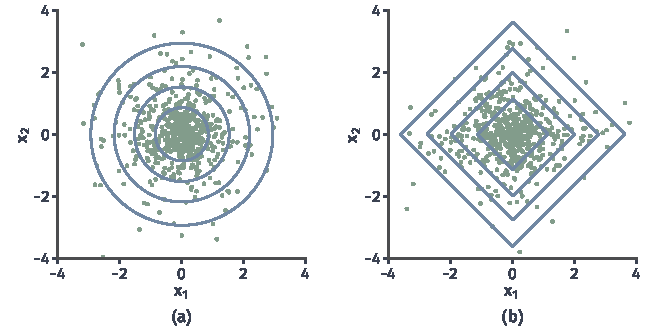
\includegraphics[width=112mm]{figures/07-probability/01-elementary-probability/matplotlib/mvd-laplace-contours/figure.pdf}
  \caption{边缘与协方差都相同的两个模型，各分量都是尺度$1/\sqrt2$的Laplace分布，协方差矩阵为$\bm{I}_2$。(a)椭圆型多元Laplace，等密度线是圆。(b)独立分量的乘积模型，等密度线是菱形。蓝线是密度等于$0.1,0.03,0.01,0.003$的等值线，绿点是各$600$个样本（种子$41$、$42$）。}
  \label{fig:mvd-laplace-contours}
\end{BookInlineFigure}

选哪一个版本，取决于数据的生成方式。各坐标的波动来自同一个源头，比如整个系统的状态忽强忽弱，椭圆型更合适；各坐标各自独立地出现尖峰，乘积模型更合适。两者都可以称为“多元Laplace”，使用时要说明采用的是哪一种构造。


\section{Dirichlet分布}
\label{sec:mvd-dirichlet}

甜品店的三种口味，选择概率$(0.5,0.3,0.2)$并不是一成不变的：天气、节日、新品都会让这天的偏好与那天不同。若把每天的偏好本身看成随机的，就得到一个随机的比例向量$\bm{P}=(P_1,P_2,P_3)^{\top}$，分量非负、和为$1$。一份混合物中各成分所占的比例，也是这样的对象。

这类对象与计数不同。多项分布中$\bm{p}$是给定的参数，随机的是计数；这里随机的是比例本身。两层可以叠加：先随机产生当天的偏好$\bm{P}$，再在给定$\bm{P}$时产生多项计数。本节只讨论比例的分布本身。由观测到的计数反过来更新对比例的认识，属于统计推断，归卷八。

一元时，第~\ref{chap:common-distributions}章的Beta分布描述$(0,1)$中的一个随机比例，另一类的比例就是它的补数。Dirichlet分布把它推广到$d$个类别。我们先说明它住在什么地方、密度相对于什么坐标，再用独立Gamma变量构造它，最后计算均值与协方差。

\subsection{单纯形上的密度}
\label{sec:mvd-dirichlet-density}

\paragraph{取值范围}
$d$个类别的比例向量取值于\term{标准单纯形}（standard simplex）
\[
 \Delta_{d-1}=\Bigl\{\bm{p}\in\mathbb{R}^{d}:\ p_i\geq0,\ \sum_{i=1}^{d}p_i=1\Bigr\} .
\]
$d=3$时它是$\mathbb{R}^{3}$中以三个坐标向量为顶点的三角形，图~\ref{fig:mvd-simplex}左侧；下标$d-1$是它的维数。

$\Delta_{d-1}$落在超平面$\sum_ip_i=1$里，$d$维体积为$0$，所以$\bm{P}$不可能有普通的$d$维密度，理由与退化高斯相同。办法是只用前$d-1$个分量作坐标，最后一个由$p_d=1-p_1-\cdots-p_{d-1}$确定。这些自由坐标取值于
\[
 T_{d-1}=\Bigl\{(p_1,\ldots,p_{d-1}):\ p_i>0,\ \sum_{i=1}^{d-1}p_i<1\Bigr\} ,
\]
$d=3$时是平面上的直角三角形，图~\ref{fig:mvd-simplex}右侧。密度就是$(P_1,\ldots,P_{d-1})$在$T_{d-1}$上的普通密度。

\begin{BookInlineFigure}
  \centering
  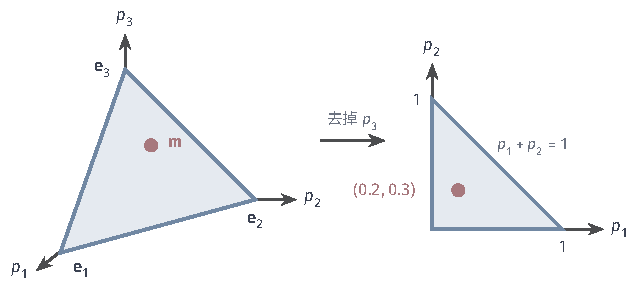
\includegraphics[width=109mm]{figures/07-probability/01-elementary-probability/tikz/mvd-simplex/figure.pdf}
  \caption{三个类别的比例。左：$\mathbb{R}^{3}$中的标准单纯形$\Delta_2$（浅蓝三角形），顶点为$\bm{e}_1,\bm{e}_2,\bm{e}_3$，红点$\bm{m}=(0.2,0.3,0.5)$。右：去掉$p_3$后的自由坐标区域$T_2$，红点是$\bm{m}$的像$(0.2,0.3)$。}
  \label{fig:mvd-simplex}
\end{BookInlineFigure}

\paragraph{密度与归一化}
Beta密度$t^{\alpha_1-1}(1-t)^{\alpha_2-1}$在$t$接近$0$时由$\alpha_1$控制，接近$1$时由$\alpha_2$控制。多个类别时，对每个比例都放一个这样的幂因子。

\begin{definition}[Dirichlet分布]
\label{def:mvd-dirichlet}
设$d\geq2$，$\bm{\alpha}=(\alpha_1,\ldots,\alpha_d)^{\top}$的各分量$\alpha_i>0$，记$\alpha_0=\alpha_1+\cdots+\alpha_d$。若随机向量$\bm{P}$取值于$\Delta_{d-1}$，且$(P_1,\ldots,P_{d-1})$在$T_{d-1}$上有密度
\begin{equation}
 f(p_1,\ldots,p_{d-1})=\frac{\Gamma(\alpha_0)}{\Gamma(\alpha_1)\cdots\Gamma(\alpha_d)}\prod_{i=1}^{d}p_i^{\alpha_i-1},\qquad p_d=1-\sum_{i=1}^{d-1}p_i ,
 \label{eq:mvd-dirichlet-density}
\end{equation}
则称$\bm{P}$服从参数为$\bm{\alpha}$的\term{Dirichlet分布}（Dirichlet distribution），记为$\bm{P}\sim\operatorname{Dir}(\bm{\alpha})$。
\end{definition}

$d=2$时，$P_1$在$(0,1)$上的密度是$\Gamma(\alpha_1+\alpha_2)/(\Gamma(\alpha_1)\Gamma(\alpha_2))\cdot p_1^{\alpha_1-1}(1-p_1)^{\alpha_2-1}$，就是$\operatorname{Beta}(\alpha_1,\alpha_2)$。第~\ref{chap:common-distributions}章的归一化等价于Beta积分
\[
 \int_0^{1}t^{a-1}(1-t)^{b-1}\,\mathrm{d}t=\frac{\Gamma(a)\Gamma(b)}{\Gamma(a+b)},\qquad a,b>0 .
\]
一般的$d$需要验证式~\eqref{eq:mvd-dirichlet-density}的积分为$1$，下面用归纳法从Beta积分推出。

\begin{lemma}[Dirichlet积分]
\label{lem:mvd-dirichlet-integral}
对$d\geq2$及正数$\alpha_1,\ldots,\alpha_d$，
\begin{equation}
 \int_{T_{d-1}}\prod_{i=1}^{d}p_i^{\alpha_i-1}\,\mathrm{d}p_1\cdots\mathrm{d}p_{d-1}=\frac{\Gamma(\alpha_1)\cdots\Gamma(\alpha_d)}{\Gamma(\alpha_0)} ,
 \label{eq:mvd-dirichlet-integral}
\end{equation}
其中$p_d=1-\sum_{i<d}p_i$。
\end{lemma}

\begin{proof}
$d=2$就是Beta积分。设结论对$d-1$成立，$d\geq3$。被积函数非负，可以先对$p_{d-1}$积分。固定$p_1,\ldots,p_{d-2}$，记$s=p_1+\cdots+p_{d-2}<1$，则$p_{d-1}$的范围是$(0,1-s)$，$p_d=1-s-p_{d-1}$。

令$p_{d-1}=(1-s)t$，$t\in(0,1)$，则$p_d=(1-s)(1-t)$，$\mathrm{d}p_{d-1}=(1-s)\,\mathrm{d}t$，于是
\[
 \int_0^{1-s}p_{d-1}^{\alpha_{d-1}-1}p_d^{\alpha_d-1}\,\mathrm{d}p_{d-1}=(1-s)^{\alpha_{d-1}+\alpha_d-1}\,\frac{\Gamma(\alpha_{d-1})\Gamma(\alpha_d)}{\Gamma(\alpha_{d-1}+\alpha_d)} .
\]

剩下对$(p_1,\ldots,p_{d-2})\in T_{d-2}$的积分，被积函数是$\prod_{i\leq d-2}p_i^{\alpha_i-1}$乘以$(1-s)^{(\alpha_{d-1}+\alpha_d)-1}$。这正是$d-1$个类别、参数为$(\alpha_1,\ldots,\alpha_{d-2},\alpha_{d-1}+\alpha_d)$时的同类积分，参数之和仍为$\alpha_0$。由归纳假设，它等于
\[
 \frac{\Gamma(\alpha_1)\cdots\Gamma(\alpha_{d-2})\,\Gamma(\alpha_{d-1}+\alpha_d)}{\Gamma(\alpha_0)} .
\]
与前一个因子相乘，$\Gamma(\alpha_{d-1}+\alpha_d)$消去，得到式~\eqref{eq:mvd-dirichlet-integral}。
\end{proof}

证明顺带说明了一件事：把最后两类合并，$(P_1,\ldots,P_{d-2},P_{d-1}+P_d)$服从$\operatorname{Dir}(\alpha_1,\ldots,\alpha_{d-2},\alpha_{d-1}+\alpha_d)$，因为对$p_{d-1}$积分后剩下的正是这个分布的密度。式~\eqref{eq:mvd-dirichlet-density}在$d$个分量间是对称的（换用另一组$d-1$个自由坐标是行列式为$\pm1$的线性换元），所以任意几类都可以合并，参数相加。反复合并，只留下第$i$类与“其余各类”，就得到边缘分布
\begin{equation}
 P_i\sim\operatorname{Beta}(\alpha_i,\ \alpha_0-\alpha_i) .
 \label{eq:mvd-dirichlet-marginal}
\end{equation}
这与多项计数合并类别后仍为多项分布是同一种结构。

\paragraph{一个例子}
取$\bm{\alpha}=(2,3,5)^{\top}$，$\alpha_0=10$。归一化常数是
\[
 \frac{\Gamma(10)}{\Gamma(2)\Gamma(3)\Gamma(5)}=\frac{9!}{1!\cdot2!\cdot4!}=\frac{362880}{48}=7560 .
\]
在$\bm{p}=(0.2,0.3,0.5)$处，密度为
\[
 7560\times0.2\times0.3^{2}\times0.5^{4}=7560\times0.001125\approx8.51 .
\]
各$\alpha_i>1$时，在约束$\sum_ip_i=1$下最大化$\ln f=\text{常数}+\sum_i(\alpha_i-1)\ln p_i$，Lagrange条件要求$(\alpha_i-1)/p_i$对各$i$相同，所以密度的最高点在$p_i=(\alpha_i-1)/(\alpha_0-d)$。这里是$(1,2,4)/7\approx(0.14,0.29,0.57)$，与均值$(0.2,0.3,0.5)$不同。

\paragraph{参数小于一的边界}
$\alpha_i<1$时因子$p_i^{\alpha_i-1}$在$p_i\to0$时趋于无穷，密度在面$p_i=0$附近无界。图~\ref{fig:mvd-dirichlet-density}(c)取$\bm{\alpha}=(0.5,0.5,0.5)^{\top}$，颜色向三条边加深。这不意味着边界上有正概率：密度只描述单位面积上的概率，无界的密度仍可以积分为有限值。

用边缘分布可以算得很具体。$\bm{\alpha}=(0.5,0.5,0.5)^{\top}$时，由式~\eqref{eq:mvd-dirichlet-marginal}，$P_1\sim\operatorname{Beta}(1/2,1)$，密度为$\tfrac12t^{-1/2}$，于是
\[
 \mathbb{P}(P_1\leq\varepsilon)=\int_0^{\varepsilon}\tfrac12t^{-1/2}\,\mathrm{d}t=\sqrt\varepsilon .
\]
$\varepsilon=0.01$时这个概率是$0.1$，比均匀分布下大得多，说明比例确实偏爱靠近边界；但它随$\varepsilon\to0$趋于$0$，所以$\mathbb{P}(P_1=0)=0$，边界上没有点质量。一般地，$\mathbb{P}(P_i\leq\varepsilon)$与$\varepsilon^{\alpha_i}$同阶。

\begin{BookInlineFigure}
  \centering
  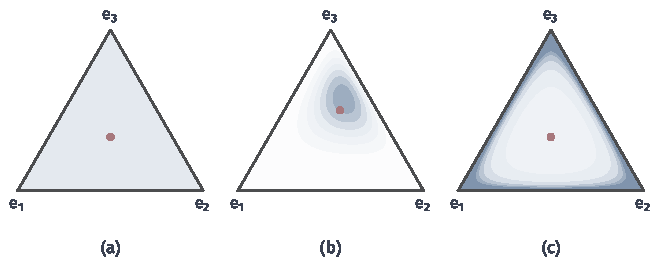
\includegraphics[width=112mm]{figures/07-probability/01-elementary-probability/matplotlib/mvd-dirichlet-density/figure.pdf}
  \caption{Dirichlet密度画在等边三角形上，顶点$\bm{e}_i$对应$p_i=1$；颜色由白到蓝表示密度由小到大，各图色阶分别设定。(a)$\bm{\alpha}=(1,1,1)$，密度恒为$2$。(b)$\bm{\alpha}=(2,3,5)$。(c)$\bm{\alpha}=(0.5,0.5,0.5)$，密度向三条边增大（颜色在$3$处截断）。红点是均值$\bm{\alpha}/\alpha_0$。}
  \label{fig:mvd-dirichlet-density}
\end{BookInlineFigure}

$\bm{\alpha}=(1,1,1)^{\top}$时密度恒为$\Gamma(3)=2$，是$T_2$上的均匀分布：三角形$T_2$的面积是$1/2$。$\alpha_i$都大于$1$时，密度在内部有唯一的峰，在边界上趋于$0$，图~\ref{fig:mvd-dirichlet-density}(b)。

\subsection{Gamma归一化}
\label{sec:mvd-gamma-normalization}

比例最自然的来源是“各部分的量除以总量”。设三种成分的量相互独立，各自是正的随机变量，把它们除以总量，就得到一个随机比例。量取Gamma分布时，比例恰好是Dirichlet分布。

\begin{theorem}[Gamma归一化]
\label{thm:mvd-gamma-normalization}
设随机变量$G_i\sim\operatorname{Gamma}(\alpha_i,\beta)$，$i=1,\ldots,d$，相互独立，速率$\beta>0$相同。令$T=G_1+\cdots+G_d$，则
\begin{equation}
 \bm{P}=\Bigl(\frac{G_1}{T},\ldots,\frac{G_d}{T}\Bigr)^{\top}\sim\operatorname{Dir}(\bm{\alpha}) ,
 \label{eq:mvd-gamma-normalization}
\end{equation}
并且$T\sim\operatorname{Gamma}(\alpha_0,\beta)$，$T$与$\bm{P}$相互独立。
\end{theorem}

证明要求出$(T,P_1,\ldots,P_{d-1})$的联合密度，这是一个$d$维到$d$维的可逆换元，在第~\ref{chap:random-variable-transformations}章用总量与比例的变换完成。这里先核对定理中各项的含义。

\paragraph{取值范围与参数}
每个$G_i$以概率$1$为正，所以$T>0$，各$P_i\in(0,1)$，且$P_1+\cdots+P_d=1$：$\bm{P}$确实落在单纯形内部。第$i$类的形状参数$\alpha_i$原样成为Dirichlet参数的第$i$个分量。形状参数越大，$G_i$越倾向于取大值，第$i$类在总量中占的比例也越大，这与下面算出的均值$\alpha_i/\alpha_0$一致。

\paragraph{共同速率被消去}
速率只是一个共同的单位。若$G\sim\operatorname{Gamma}(\alpha,\beta)$，对$x>0$代换$h=\beta g$，
\[
 \mathbb{P}(\beta G\leq x)=\int_0^{x/\beta}\frac{\beta^{\alpha}g^{\alpha-1}\mathrm{e}^{-\beta g}}{\Gamma(\alpha)}\,\mathrm{d}g=\int_0^{x}\frac{h^{\alpha-1}\mathrm{e}^{-h}}{\Gamma(\alpha)}\,\mathrm{d}h ,
\]
所以$\beta G\sim\operatorname{Gamma}(\alpha,1)$。于是可以写$G_i=H_i/\beta$，$H_i\sim\operatorname{Gamma}(\alpha_i,1)$相互独立，而
\[
 \frac{G_i}{T}=\frac{H_i/\beta}{\sum_jH_j/\beta}=\frac{H_i}{\sum_jH_j} .
\]
比例与$\beta$无关。共同速率只改变各部分的单位，不改变各部分之间的相对大小。

如果各$G_i$的速率不同，速率就不能约去，比例一般不是Dirichlet分布。图~\ref{fig:mvd-gamma-normalization}以$\bm{g}=(1.2,0.6,2.2)$为例：总量为$4$，比例为$(0.3,0.15,0.55)$；所有量同时加倍（相当于速率减半）后总量为$8$，比例不变。

\begin{BookInlineFigure}
  \centering
  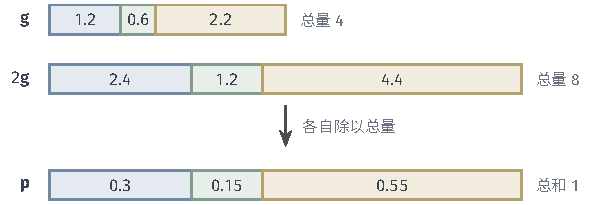
\includegraphics[width=97mm]{figures/07-probability/01-elementary-probability/tikz/mvd-gamma-normalization/figure.pdf}
  \caption{Gamma归一化的一个取值。三种成分的量$\bm{g}=(1.2,0.6,2.2)$（第一行），全部加倍得$2\bm{g}$（第二行）；除以各自的总量$4$与$8$后得到同一个比例向量$\bm{p}=(0.3,0.15,0.55)$（第三行）。}
  \label{fig:mvd-gamma-normalization}
\end{BookInlineFigure}

\paragraph{比例之间为什么相关}
$G_1,\ldots,G_d$相互独立，比例却通过共同的分母联系在一起：某一类的量偏大，总量随之变大，其他各类的比例就被压低。这与多项计数的负相关来源相似，都是“总和固定”在起作用。

定理~\ref{thm:mvd-gamma-normalization}还给出了生成Dirichlet样本的方法：独立地生成$d$个Gamma变量，第$i$个的形状参数为$\alpha_i$、速率为$1$，再各自除以它们的和。下一小节图中的模拟样本就是这样得到的，更多的生成方法在第~\ref{chap:sample-generation}章讨论。

\subsection{均值与协方差}
\label{sec:mvd-dirichlet-moments}

Dirichlet积分把矩的计算变成参数的移位：乘以$p_i$，只是把$\alpha_i$加$1$。对非负整数$r_1,\ldots,r_d$，记$r=\sum_ir_i$，由式~\eqref{eq:mvd-dirichlet-integral}，
\begin{equation}
 \mathbb{E}\Bigl[\prod_{i=1}^{d}P_i^{r_i}\Bigr]=\frac{\Gamma(\alpha_0)}{\Gamma(\alpha_0+r)}\prod_{i=1}^{d}\frac{\Gamma(\alpha_i+r_i)}{\Gamma(\alpha_i)} .
 \label{eq:mvd-dirichlet-moments}
\end{equation}
这里的乘积包括$P_d$，因为$p_d$在被积函数中本来就以幂的形式出现。

\begin{theorem}[Dirichlet的均值与协方差]
\label{thm:mvd-dirichlet-cov}
设$\bm{P}\sim\operatorname{Dir}(\bm{\alpha})$，记$m_i=\alpha_i/\alpha_0$，$\bm{m}=(m_1,\ldots,m_d)^{\top}$。则$\mathbb{E}[\bm{P}]=\bm{m}$，并且
\begin{equation}
 \operatorname{Cov}(\bm{P})=\frac{1}{\alpha_0+1}\bigl(\operatorname{diag}(\bm{m})-\bm{m}\bm{m}^{\top}\bigr) ,
 \label{eq:mvd-dirichlet-cov}
\end{equation}
即$\operatorname{Var}(P_i)=m_i(1-m_i)/(\alpha_0+1)$，$i\neq j$时$\operatorname{Cov}(P_i,P_j)=-m_im_j/(\alpha_0+1)$。
\end{theorem}

\begin{proof}
在式~\eqref{eq:mvd-dirichlet-moments}中用$\Gamma(x+1)=x\Gamma(x)$。只取$r_i=1$，得$\mathbb{E}[P_i]=\alpha_i/\alpha_0$。取$r_i=2$或$r_i=r_j=1$（$i\neq j$），得
\[
 \mathbb{E}[P_i^{2}]=\frac{\alpha_i(\alpha_i+1)}{\alpha_0(\alpha_0+1)},\qquad \mathbb{E}[P_iP_j]=\frac{\alpha_i\alpha_j}{\alpha_0(\alpha_0+1)} .
\]

方差为
\[
 \begin{aligned}
  \operatorname{Var}(P_i)&=\frac{\alpha_i(\alpha_i+1)}{\alpha_0(\alpha_0+1)}-\frac{\alpha_i^{2}}{\alpha_0^{2}}
  =\frac{\alpha_i\bigl[(\alpha_i+1)\alpha_0-\alpha_i(\alpha_0+1)\bigr]}{\alpha_0^{2}(\alpha_0+1)}\\
  &=\frac{\alpha_i(\alpha_0-\alpha_i)}{\alpha_0^{2}(\alpha_0+1)} ,
 \end{aligned}
\]
即$m_i(1-m_i)/(\alpha_0+1)$。协方差为
\[
 \operatorname{Cov}(P_i,P_j)=\frac{\alpha_i\alpha_j}{\alpha_0(\alpha_0+1)}-\frac{\alpha_i\alpha_j}{\alpha_0^{2}}=-\frac{\alpha_i\alpha_j}{\alpha_0^{2}(\alpha_0+1)} .
\]
\end{proof}

用边缘分布核对一下。由式~\eqref{eq:mvd-dirichlet-marginal}，$P_i\sim\operatorname{Beta}(\alpha_i,\alpha_0-\alpha_i)$；按第~\ref{chap:common-distributions}章的Beta公式，均值是$\alpha_i/\alpha_0$，方差是
\[
 \frac{\alpha_i(\alpha_0-\alpha_i)}{\alpha_0^{2}(\alpha_0+1)} ,
\]
与定理一致。也可以用定理~\ref{thm:mvd-gamma-normalization}核对均值：$G_i=TP_i$，而$T$与$\bm{P}$独立，所以
\[
 \frac{\alpha_i}{\beta}=\mathbb{E}[G_i]=\mathbb{E}[T]\,\mathbb{E}[P_i]=\frac{\alpha_0}{\beta}\,\mathbb{E}[P_i] ,
\]
即$\mathbb{E}[P_i]=\alpha_i/\alpha_0$。

取$\bm{\alpha}=(2,3,5)^{\top}$，$\bm{m}=(0.2,0.3,0.5)^{\top}$，$\alpha_0+1=11$。代入式~\eqref{eq:mvd-dirichlet-cov}，
\[
 \operatorname{Cov}(\bm{P})=\frac{1}{11}\begin{bmatrix}0.16&-0.06&-0.10\\-0.06&0.21&-0.15\\-0.10&-0.15&0.25\end{bmatrix}\approx\begin{bmatrix}0.0145&-0.0055&-0.0091\\-0.0055&0.0191&-0.0136\\-0.0091&-0.0136&0.0227\end{bmatrix} .
\]
三个比例两两负相关，每行之和为$0$。

\paragraph{总和约束与奇异协方差}
行和为$0$的原因与多项分布相同：$\operatorname{diag}(\bm{m})-\bm{m}\bm{m}^{\top}$乘以$\bm{1}$得$\bm{m}-\bm{m}=\bm{0}$，对应$\operatorname{Var}(P_1+\cdots+P_d)=0$。各$m_i>0$，所以与多项分布一样，这个矩阵的秩是$d-1$，与单纯形的维数一致。所有比例两两负相关：一个比例变大，其余比例的总和必须变小。

\paragraph{集中程度}
式~\eqref{eq:mvd-dirichlet-cov}把参数分成两部分：方向$\bm{m}=\bm{\alpha}/\alpha_0$决定均值，总和$\alpha_0$决定比例围绕均值的集中程度，协方差与$\alpha_0+1$成反比。$\alpha_0$因此称为\term{集中参数}（concentration parameter）。

固定$\bm{m}=(0.2,0.3,0.5)^{\top}$，让$\alpha_0$取$1,10,100$，$\operatorname{Var}(P_1)=0.16/(\alpha_0+1)$分别是$0.08$、$0.0145$、$0.0016$。图~\ref{fig:mvd-dirichlet-concentration}画出对应的样本。$\alpha_0=1$时各$\alpha_i<1$，样本挤到边和顶点附近，即某一两类占了绝大部分；$\alpha_0=100$时样本紧紧围着$\bm{m}$。

\begin{BookInlineFigure}
  \centering
  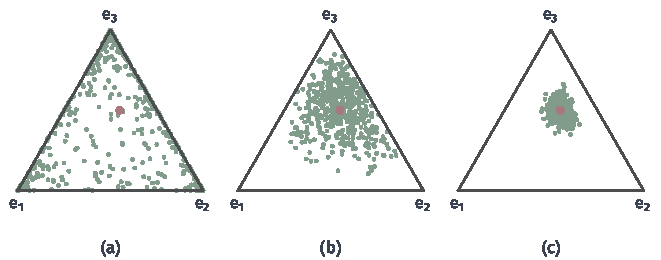
\includegraphics[width=112mm]{figures/07-probability/01-elementary-probability/matplotlib/mvd-dirichlet-concentration/figure.pdf}
  \caption{均值固定为$\bm{m}=(0.2,0.3,0.5)$（红点）、集中参数不同的Dirichlet样本，各$500$个，用Gamma归一化生成。(a)$\alpha_0=1$，种子$51$；(b)$\alpha_0=10$，种子$52$；(c)$\alpha_0=100$，种子$53$。三组样本中$P_1$的样本方差分别约为$0.089$、$0.014$、$0.0016$。}
  \label{fig:mvd-dirichlet-concentration}
\end{BookInlineFigure}


\section{模型比较}
\label{sec:mvd-comparison}

面对一组多元记录，选模型的第一步是看记录的类型：类别计数、实值观测还是组成比例。同一类型中的几个模型，均值甚至协方差可以完全相同，联合规律却不同。本节把前面的结果并排放在一起（表~\ref{tab:mvd-models}），说明哪些特征能区分它们，为什么不能只凭边缘或协方差互相替代。

\begin{BookInlineTable}
  \centering
  \small
  \begin{tabular}{llll}
    \toprule
    模型 & 取值范围 & 协方差矩阵 & 依赖的来源\\
    \midrule
    $\operatorname{Mult}(n,\bm{p})$ & 和为$n$的格点 & $n(\operatorname{diag}\bm{p}-\bm{p}\bm{p}^{\top})$ & 总数固定\\
    多元超几何 & 同上，且$k_i\leq K_i$ & 上式乘$\frac{M-n}{M-1}$ & 总数固定，不放回\\
    $\mathcal{N}(\bm{\mu},\bm{\Sigma})$ & $\bm{\mu}$加$\bm{\Sigma}$的列空间 & $\bm{\Sigma}$ & 共享的高斯分量\\
    多元t & $\mathbb{R}^{d}$ & $\frac{\nu}{\nu-2}\bm{\Sigma}$（$\nu>2$） & 同上，加共同尺度\\
    多元Laplace & $\mathbb{R}^{d}$ & $\bm{\Sigma}$ & 同上，加共同尺度\\
    $\operatorname{Dir}(\bm{\alpha})$ & 单纯形$\Delta_{d-1}$ & $\frac{\operatorname{diag}\bm{m}-\bm{m}\bm{m}^{\top}}{\alpha_0+1}$ & 总和为$1$\\
    \bottomrule
  \end{tabular}
  \caption{本章五个模型及多元超几何分布的取值范围、协方差与依赖来源。多元t与多元Laplace取$\bm{\Sigma}$正定；Dirichlet中$\bm{m}=\bm{\alpha}/\alpha_0$。}
  \label{tab:mvd-models}
\end{BookInlineTable}

\paragraph{计数与比例}
多项分布与多元超几何分布的均值相同，协方差只差因子$(M-n)/(M-1)$；后者还多了上限$k_i\leq K_i$。抽样比例$n/M$小时两者可以互换，抽样比例大时多项分布会高估波动，并给不可能的计数分配概率。

计数比例$\bm{N}/n$与Dirichlet比例更容易混淆。由定理~\ref{thm:mvd-multinomial-moments}，$\bm{N}\sim\operatorname{Mult}(n,\bm{m})$时
\[
 \operatorname{Cov}(\bm{N}/n)=\frac1n\bigl(\operatorname{diag}(\bm{m})-\bm{m}\bm{m}^{\top}\bigr) .
\]
与式~\eqref{eq:mvd-dirichlet-cov}比较，取$n=\alpha_0+1$，两者的均值和协方差完全相同。例如$\bm{m}=(0.2,0.3,0.5)^{\top}$时，$\operatorname{Mult}(11,\bm{m})$的计数比例与$\operatorname{Dir}(2,3,5)$有同样的前两阶矩。

可是两个分布截然不同。$\bm{N}/11$只取$1/11$的整数倍，以正概率恰好等于$0$，例如$\mathbb{P}(N_1=0)=0.8^{11}\approx0.086$；Dirichlet比例在单纯形内部连续取值，$\mathbb{P}(P_1=0)=0$。前两阶矩相同，不足以让一个代替另一个。

\paragraph{实值观测}
多元高斯、多元t与多元Laplace都是椭圆分布：给定$\bm{\mu}$和$\bm{\Sigma}$，三者的等密度面是同一族椭球。区别在于沿椭球向外的衰减，以及有没有共同尺度。为了公平比较，把三者都调到均值为$\bm{0}$、协方差为$\bm{I}_2$：高斯取$\bm{\Sigma}=\bm{I}$，Laplace取$\bm{\Sigma}=\bm{I}$，$\nu=5$的t分布取$\bm{\Sigma}=\tfrac35\bm{I}$，由式~\eqref{eq:mvd-t-cov}，它的协方差也是$\bm{I}$。

第一个差别在边缘的尾部。$\mathbb{P}(\lvert X_1\rvert>3)$在高斯下约为$0.0027$，在Laplace下为$\mathrm{e}^{-3\sqrt2}\approx0.0144$，在t下约为$0.0117$，后两者是高斯的四到五倍，图~\ref{fig:mvd-model-tails}(a)。更远处差别更大：Laplace的尾部按指数衰减，t的尾部按$r^{-5}$衰减，最终比任何指数都慢。

第二个差别在于大值是否一起出现。三者的协方差都是$\bm{I}$，分量两两不相关。若分量独立，$\mathbb{P}(\lvert X_1\rvert>r,\lvert X_2\rvert>r)$应等于$\mathbb{P}(\lvert X_1\rvert>r)^{2}$。对正态尺度混合$\bm{X}=\sqrt{V}\bm{Z}$，先固定$V$再积分，两个概率都可以化为一元积分：记$h(v)=\mathbb{P}(\lvert Z_1\rvert>r/\sqrt v)$，则
\[
 \mathbb{P}(\lvert X_1\rvert>r)=\mathbb{E}[h(V)],\qquad \mathbb{P}(\lvert X_1\rvert>r,\ \lvert X_2\rvert>r)=\mathbb{E}[h(V)^{2}] .
\]

由$\mathbb{E}[h(V)^{2}]\geq(\mathbb{E}[h(V)])^{2}$，比值总不小于$1$，只有$V$为常数时取等号。图~\ref{fig:mvd-model-tails}(b)画出这个比值：高斯恒为$1$；$r=3$时Laplace约为$6.2$，t约为$11.7$。两个分量同时超过$3$的机会，是“假装独立”时估计的六到十几倍。前两节的乘积模型边缘相同、协方差相同，这个比值却恒为$1$。

\begin{BookInlineFigure}
  \centering
  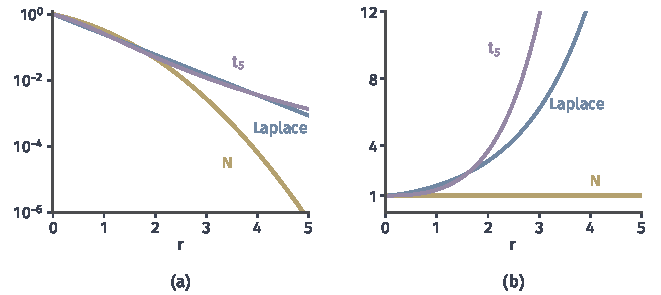
\includegraphics[width=112mm]{figures/07-probability/01-elementary-probability/matplotlib/mvd-model-tails/figure.pdf}
  \caption{均值为$\bm{0}$、协方差为$\bm{I}_2$的三个椭圆模型：高斯（黄）、多元Laplace（蓝）、$\nu=5$的多元t（紫，尺度矩阵$\tfrac35\bm{I}$）。(a)边缘尾概率$\mathbb{P}(\lvert X_1\rvert>r)$，纵轴取对数。(b)联合超越比$\mathbb{P}(\lvert X_1\rvert>r,\lvert X_2\rvert>r)/\mathbb{P}(\lvert X_1\rvert>r)^{2}$，独立时恒为$1$。曲线由对共同尺度的精确密度数值积分得到。}
  \label{fig:mvd-model-tails}
\end{BookInlineFigure}

\paragraph{不相关与独立}
三种实值模型对“不相关能否推出独立”给出不同回答。联合高斯时，零交叉协方差推出独立，定理~\ref{thm:mvd-gaussian-independence}。多元t与多元Laplace中，即使尺度矩阵是对角的，共同尺度也使分量相关于各自的大小，零协方差不推出独立。$(Z,SZ)$说明另一种失效：每个分量都是高斯，但向量不联合高斯，定理同样不适用。

\paragraph{矩与支撑}
矩的存在条件也不同。高斯与Laplace的各阶矩都有限；t分布只有低于$\nu$阶的矩，$\bm{\Sigma}$只在$\nu>2$时通过$\nu/(\nu-2)$与协方差相连。支撑维数则由约束决定：计数与比例都受一条线性约束，住在$d-1$维的格点或单纯形上；退化高斯受$d-r$条线性约束，住在$r$维平面上。凡是有约束的模型，协方差矩阵都奇异，零空间正对应约束方向。

这些比较说明，选择多元模型时要同时核对四件事：取值范围与约束，边缘的尾部，依赖的来源，需要的矩是否存在。只核对均值与协方差，会把本质不同的模型当成可以互换的。


\section{本章小结}
\label{sec:mvd-summary}

本章从试验机制和取值范围出发，写出了五种常见的多元分布，并追问各自的依赖从哪里来。四种构造方式贯穿全章：独立试验的计数，标准高斯向量的仿射像，高斯向量乘以共同的随机尺度，独立Gamma变量除以总量。

计数模型来自独立试验或不放回抽样。多项分布由逐次独立、单次互斥得到协方差$n(\operatorname{diag}\bm{p}-\bm{p}\bm{p}^{\top})$；多元超几何分布的均值相同，协方差多乘有限总体因子$(M-n)/(M-1)$，抽样比例小时可以用多项分布近似。总数固定使协方差矩阵奇异，各类计数两两负相关。

多元高斯定义为$\bm{\mu}+\bm{A}\bm{Z}$的分布，它只由$\bm{\mu}$与$\bm{\Sigma}=\bm{A}\bm{A}^{\top}$决定，在仿射变换下封闭，边缘只需取子块。$\bm{\Sigma}$正定时有满维密度，等密度面是马氏距离的椭球；$\bm{\Sigma}$奇异时分布落在低维平面上。分块后，条件均值是观测的仿射函数，条件协方差是与观测无关的Schur补；残差与观测独立，这一正交分解也给出了高斯样本平均与残差平方和的独立性。零交叉协方差推出独立，只在联合高斯时成立。

多元t与多元Laplace把高斯的固定尺度换成共同的随机尺度：t用$\sqrt{\nu/U}$，尾部按负幂衰减，只有低于$\nu$阶的矩，$\bm{\Sigma}$是尺度矩阵；Laplace用$\sqrt W$，边缘是一元Laplace，各阶矩有限，$\bm{\Sigma}$就是协方差。两者都是椭圆分布，尺度矩阵为对角时分量不相关却不独立，大值倾向于同时出现；改用各分量独立的尺度，得到边缘与协方差相同而联合规律不同的乘积模型。

Dirichlet分布描述单纯形上的随机比例，密度相对于$d-1$个自由坐标给出，参数小于一时在边界附近无界却没有点质量。它可以由同速率独立Gamma变量归一化得到，边缘是Beta分布，均值为$\bm{\alpha}/\alpha_0$，协方差与$\alpha_0+1$成反比，并因总和为$1$而奇异。

本章多次用到“已知输入的分布，求输出的分布”：仿射像的密度、尺度混合的密度、Gamma归一化的联合密度。第~\ref{chap:random-variable-transformations}章把这些具体计算整理成一般的变换方法，补全了本章留给它的换元证明。

